\documentclass[journal=cic,version=preprint]{iacrj}

\license{CC-BY-4.0}

\title[running={The Root Hermite Factor Is Blind}]{The Root Hermite Factor Is Blind: Structural Differences in Lattice Reduction Revealed by the Li--Nguyen Rankin Profile}

\addauthor[surname = {Chambers-Bourgeois},
           email   = {brendanchambersbou@gmail.com},
           orcid   = {0009-0004-2609-0822},
           inst    = {1}
          ]{Brendan Chambers-Bourgeois}

\addaffiliation[country={Australia},
                city={Melbourne}]{Independent Researcher}

\keywords{lattice reduction, BKZ, SD-BKZ, Rankin profile, Li--Nguyen, Root Hermite Factor, LWE, dynamical systems}

\begin{document}
\maketitle

\begin{abstract}
The Root Hermite Factor (RHF), the dominant quality metric for lattice basis reduction, is structurally blind to meaningful differences between reduced bases. Comparing BKZ against self-dual BKZ (SD-BKZ) across more than 4{,}500 seeds on LWE-Kannan embedding lattices ($n = 50$--$150$, $\beta = 20, 30, 40$), we find that RHF differences are below $10^{-6}$ in all groups without outlier seeds, while the Li--Nguyen Rankin profile distance $d(\mathrm{LN})$ reveals statistically significant gaps (Cohen's $d$ up to 9.6). The SD-BKZ advantage is non-monotonic: it rises with dimension, peaks at a block-size-dependent dimension ($\beta=20$ at $n=90$ with 0.48 nats; $\beta=30$ at $n=100$ with 1.35 nats; $\beta=40$ at $n=110$ with 1.16 nats), then declines into negative territory where the backward pass becomes actively harmful ($\beta=30$ reaches $-0.40$ nats at $n=150$ with 0\% win rate; $\beta=40$ collapses to $-1.32$ nats at $n=130$). Giving BKZ $3\times$ the tour budget does not close the gap at $\beta=30$ (0/400 seeds across four dimensions), establishing this as a capability difference rather than a speed difference at $\beta\geq 30$; at $\beta=20$, extra tours partially compensate (67\% of the gap closed). This behaviour, governed by the interaction of block size, dimension, and convergence depth, is invisible to RHF. These findings suggest that prior RHF-only evaluations may have missed structural quality differences between reduction algorithms. All experiments are fully reproducible via a containerised benchmark.
\end{abstract}

\section{Introduction}
\label{sec:intro}

Since Gama and Nguyen's influential study~\cite{EC:GamNgu08}, the Root Hermite Factor (RHF) has served as the standard scoreboard for comparing lattice basis reduction algorithms. Every major empirical evaluation of BKZ, its variants, and competing algorithms reports RHF as the primary quality metric. Security estimates for lattice-based cryptographic schemes, including the NIST post-quantum standard ML-KEM, rely on predictions of achievable RHF to set parameter sizes.

We pose a simple question: \emph{is RHF actually capturing everything that matters about a reduced basis?}

We answer in the negative. By comparing standard BKZ against self-dual BKZ (SD-BKZ)~\cite{EC:MicWal16} using the Li--Nguyen Rankin profile distance $d(\mathrm{LN})$---a metric derived from the dynamical systems analysis of BKZ~\cite{EPRINT:LiNgu20}---we show that SD-BKZ produces bases that are measurably and consistently closer to the theoretical fixed point predicted by Li and Nguyen (whether SD-BKZ shares this fixed point or approaches a distinct attractor is theoretically open --- see Section~\ref{sec:limitations}). This structural improvement is entirely invisible to RHF: across more than 4{,}500 completed seeds, the mean RHF difference between the two algorithms is below $10^{-6}$ in every group without outlier seeds, while $d(\mathrm{LN})$ reveals advantages of 0.1--1.3 nats (natural log units) with win rates of 90--100\%.

This is not a paper about SD-BKZ being ``better'' than BKZ in an absolute sense---it is approximately $2.5\times$ slower. Rather, it makes two contributions. First, it demonstrates that the metric the community uses to evaluate reduction quality is incomplete: RHF cannot distinguish between two algorithms that produce structurally different bases. Second, by measuring that structural difference at scale, it reveals a rich phenomenology---non-monotonic dimension scaling, block-size-dependent peaks, and a sharp $\beta=40$ cliff---that is entirely invisible to RHF and that has never been empirically characterised.

White~\cite{White26} explored dynamic block size strategies within the Li--Nguyen framework, motivating the question of whether the Rankin profile distance could serve as a more discriminating benchmark than RHF for comparing reduction algorithm variants. The present work pursues that question directly.

\begin{table}[tbp]
\centering
\caption{The same experiment yields opposite conclusions depending on the metric.\label{tab:metric-split}}
\begin{tabular}{p{3.2cm}p{8.5cm}}
\hline
\textbf{Evaluation metric} & \textbf{Conclusion drawn} \\
\hline
RHF only & No significant difference. SD-BKZ offers no advantage over BKZ for the additional runtime cost. \\
$d(\mathrm{LN})$ & SD-BKZ produces structurally superior bases in $>95\%$ of trials. The improvement is in the interior basis structure, invisible to the first vector length. \\
\hline
\end{tabular}
\end{table}

Our contributions are:

\textbf{(1)} A demonstration that RHF is structurally blind to the difference between BKZ and SD-BKZ output bases, despite a consistent and statistically significant gap in Rankin profile quality.

\textbf{(2)} The first empirical application of the Li--Nguyen $d(\mathrm{LN})$ metric as a scalar convergence benchmark for lattice reduction, enabling paired statistical comparison between algorithm variants.

\textbf{(3)} A large-scale, multi-seed comparison of SD-BKZ versus BKZ on LWE-Kannan embedding lattices, building on Micciancio and Walter's~\cite{EC:MicWal16} original 10-instance evaluation with more than 4{,}500 statistically independent trials.

\textbf{(4)} Discovery of a non-monotonic scaling pattern governed by three interacting factors: block size, lattice dimension, and convergence depth. The peak dimension is block-size-dependent: $\beta=20$ peaks at $n=90$ (0.48 nats), $\beta=30$ peaks at $n=100$ (1.35 nats), $\beta=40$ peaks at $n=110$ (1.16 nats). All three block sizes eventually decline into negative territory, where the backward pass is actively harmful. At $\beta=40$, $n=120$, the advantage is negative despite a favourable $\beta/n$ ratio, revealing convergence depth as a third governing parameter.

\textbf{(5)} Structural evidence that the SD-BKZ advantage is a capability difference, not a speed difference: BKZ given $3\times$ the standard tour budget cannot close the gap at $\beta=30$ (0/400 seeds across four dimensions), while at $\beta=20$ the gap partially closes (Section~\ref{sec:capability}). A spatial decomposition shows the improvement concentrates in the middle third of the Rankin profile, consistent with the backward pass providing optimisation pressure from a direction standard BKZ cannot reach (Section~\ref{sec:spatial}).

\section{Background}
\label{sec:background}

\subsection{BKZ and Self-Dual BKZ}

The BKZ algorithm~\cite{MathProg:SchEuc94} performs lattice basis reduction by sliding a window of size $\beta$ over the Gram--Schmidt orthogonalisation, calling an SVP oracle within each local block, and updating the basis. One complete pass constitutes a ``tour.'' BKZ 2.0~\cite{AC:CheNgu11} added practical improvements including pruned enumeration and recursive preprocessing; these are incorporated in modern implementations including fplll.

SD-BKZ~\cite{EC:MicWal16} augments each forward tour with a backward pass on the reversed dual basis. This can be understood as: (1) run a forward BKZ tour, (2) compute the reversed dual basis, (3) repeat. The backward pass improves the interior structure of the basis---particularly the middle portion of the Gram--Schmidt profile, which the forward-only pass is slowest to reach. In fplll, SD-BKZ is activated via the \texttt{BKZ.SD\_VARIANT} flag, which implements Algorithm~6 of~\cite{EC:MicWal16}. Both variants share the same SVP oracle and preprocessing; the only difference is the additional backward pass. For an accessible introduction to the dynamical systems perspective on SD-BKZ, see Walter's blog series at the Simons Institute~\cite{Walter20blog}.

Albrecht et al.~\cite{C:ABFKSW20} exploited the predicted geometry of SD-BKZ-reduced bases---specifically, that the initial Gram--Schmidt norms more closely follow Schnorr's Geometric Series Assumption---to achieve faster enumeration. Their work takes the theoretical SD-BKZ geometry as a given; the present work provides the first large-scale empirical confirmation that this geometric improvement is real and consistent.

\subsection{The Li--Nguyen Fixed Point and $d(\mathrm{LN})$}

Li and Nguyen~\cite{EPRINT:LiNgu20} provided a complete dynamical systems analysis of BKZ, building on the earlier framework of Hanrot, Pujol and Stehl\'{e}~\cite{C:HanPujSte11}, proving convergence to a unique fixed-point Rankin profile. The Rankin profile of a basis with Gram--Schmidt log-norms $\ln\|b^*_i\|$ is
\begin{equation}
R_k = \sum_{i=1}^{k} \ln\|b^*_i\| - \frac{k}{d} \sum_{i=1}^{d} \ln\|b^*_i\|
\end{equation}
where $d$ is the dimension over which the profile is computed. For LWE-Kannan embedding lattices with $m=2n$ samples, the full lattice dimension is $3n+1$, but the first $2n$ basis vectors correspond to the sample structure; BKZ reduction acts meaningfully only on the remaining $n+1$ vectors (the ``active block'' containing the secret/error embedding). We compute the Rankin profile and $d(\mathrm{LN})$ over this active block ($d=n+1$), which is standard practice for LWE-Kannan lattices. The fixed-point profile $R^*$ is determined by $\beta$ and $d$ via a closed-form expression combining the GSA slope with the Hermite bound offset (Li--Nguyen Equation~2). We define the convergence distance
\begin{equation}
d(\mathrm{LN}) = \frac{1}{d} \sum_{k=1}^{d} \left| R_k - R^*_k \right|
\end{equation}
where the distance is measured in nats (natural logarithm units), following from the use of $\ln$ in the Rankin profile definition. We use the $L^1/n$ (mean absolute error) norm rather than $L^2$ or $L^\infty$ because it weights all positions in the profile equally, avoiding undue sensitivity to a single large deviation at one index (as $L^\infty$ would) or quadratic amplification of outlier positions (as $L^2$ would). Lower $d(\mathrm{LN})$ indicates a basis closer to the fixed point. The advantage is defined as $d(\mathrm{LN})_{\mathrm{BKZ}} - d(\mathrm{LN})_{\mathrm{SD\text{-}BKZ}}$; positive values indicate SD-BKZ is closer. We measure distance to the BKZ fixed point for both algorithms; this choice and its implications are discussed in Section~\ref{sec:limitations}.

Profile-based analysis of BKZ is well established: the Chen--Nguyen BKZ simulator~\cite{AC:CheNgu11} predicts Gram--Schmidt profiles heuristically, Yu and Ducas~\cite{SAC:YuDuc17} studied second-order statistical behaviour of GS log-norm profiles, and Ducas~\cite{EC:Ducas18} exploited profile shape to obtain ``dimensions for free'' in sieving-based SVP solving. The $d(\mathrm{LN})$ metric captures the full Rankin profile shape, including deviations at both the head and tail of the basis---such as the ``head concavity'' phenomenon characterised by Bai, Stehl\'{e} and Wen~\cite{AC:BaiSteWen18}, where the first few Gram--Schmidt norms are shorter than the Chen--Nguyen simulator predicts. Our contribution is not profile-based analysis per se, but operationalising the Li--Nguyen fixed point as a single scalar convergence benchmark, enabling paired statistical comparison between algorithm variants at scale.

\subsection{Root Hermite Factor}

The Root Hermite Factor $\delta = (\|b_1\| / \mathrm{vol}(L)^{1/d})^{1/d}$ is a scalar metric that depends only on the length of the shortest basis vector relative to the lattice volume. Our implementation stores and reports the uprooted Hermite Factor $\mathrm{HF} = \delta^d$ directly (since $\mathrm{RHF} = \mathrm{HF}^{1/d}$, a monotone transformation, either metric ranks algorithms identically).\footnote{Our implementation computes the Hermite Factor (without the outer $1/d$ exponent); since $\mathrm{RHF} = \mathrm{HF}^{1/d}$ is a monotone transformation, the conclusions hold for both metrics.} It captures nothing about the interior structure of the basis; the Gram--Schmidt vectors $b^*_2$ through $b^*_d$ are invisible to it. As we demonstrate, this makes it fundamentally unable to detect the type of structural improvement SD-BKZ provides.

\section{Experimental Design}
\label{sec:design}

\subsection{Scale and Justification}

The most recent published empirical comparison of SD-BKZ against BKZ is~\cite{EC:MicWal16}, which used 10 instances. We extend this by a factor of $400\times$, running more than 4{,}500 independent trials across a systematic parameter grid (3{,}388 in the main sweep plus verification and extended-tour experiments). This scale enables statistical inference---confidence intervals, effect sizes, per-seed distributions---that is impossible with 10 instances. Multi-seed statistical benchmarking of BKZ at this scale is rare in the literature; no prior study has combined SD-BKZ with the Li--Nguyen Rankin profile metric.

\subsection{Lattice Construction}

We generate LWE instances with secret dimension $n$ and modulus $q=97$. The small modulus is a deliberate choice: it keeps lattice entries small and individual reductions fast (minutes to hours rather than days), enabling the large seed count necessary for statistical analysis. We acknowledge this is far from cryptographic moduli (e.g., $q=3329$ for ML-KEM); testing at least one parameter group at a larger $q$ would strengthen generalisability. A 20-seed verification group at $q=3329$ (the ML-KEM modulus) at $n=50$, $\beta=30$ produced a mean advantage of 0.437 nats (std 0.143, 100\% win rate, Cohen's $d=3.06$, $p=2.8\times 10^{-11}$), consistent with the $q=97$ results (0.405 nats). A two-sample $t$-test found no significant difference between the two moduli ($p=0.37$). Additional verification at $n=70$ and $n=80$ (20 seeds each, $\beta=30$, 100\% win) confirmed the effect holds across dimensions. At $n=100$, a larger verification revealed a numerical instability in fplll's GSO computation (Section~\ref{sec:q3329}). The sample dimension is $m=2n$, and the Kannan embedding produces a lattice of full dimension $m+n+1 = 3n+1$; as defined above, $d(\mathrm{LN})$ is normalised over the active block ($d=n+1$), not this full dimension. For each $(n, \beta, \mathrm{seed})$ triple, both BKZ and SD-BKZ are run on the same initial lattice generated from a fixed random seed, ensuring pairwise comparison.

\subsection{Parameter Grid}

\begin{sloppypar}
Dimensions: $n \in \{50, 60, 70, 80, 90, 100, 110, 120, 130, 140, 150\}$. Block sizes: $\beta \in \{20, 30, 40\}$. Seeds: 100 per $(n, \beta)$ pair (122 for four variance-filled groups). Total: 3{,}388 runs. Tours per reduction: 50 ($\beta=20$), 70 ($\beta=30$), 100 ($\beta=40$). MPFR precision: 250 bits.
\end{sloppypar}

\subsection{Implementation}

All reductions use fplll~\cite{fplll} 5.5.0 via fpylll~\cite{fpylll} 0.6.4. Standard BKZ uses \texttt{BKZ.MAX\_LOOPS\,|\,BKZ.AUTO\_ABORT}. SD-BKZ adds \texttt{BKZ.SD\_VARIANT}. No custom reduction code is used; both variants call the same fplll C++ library with the same SVP oracle and preprocessing. BKZ 2.0 features (recursive preprocessing) are included in fplll and are present in both variants. The $d(\mathrm{LN})$ metric has been verified to machine precision (float64) against a second, independently written implementation by the author.

Early exit occurs when the mean absolute Rankin profile change between consecutive tours falls below $10^{-6}$. In practice, this condition was triggered in only 1 of 6{,}776 algorithm runs (a single BKZ run at $n=50$, $\beta=20$). All other runs reached the tour limit, confirming that all pairwise comparisons occur at identical tour counts. This also implies the reported $d(\mathrm{LN})$ advantages are conservative: both algorithms are still improving at the tour limit, and since SD-BKZ improves faster, additional tours would be expected to widen rather than narrow the gap.

SD-BKZ is consistently slower than BKZ due to the additional backward pass. Table~\ref{tab:runtime} reports mean wall-clock runtimes for all complete 100-seed groups. The ratio ranges from $2.72\times$ ($n=70$, $\beta=30$) to $2.00\times$ ($n=140$, $\beta=20$), with a systematic compression at higher dimensions: the overhead drops from ${\sim}2.6\times$ at $n=50$--$90$ to ${\sim}2.0$--$2.4\times$ at $n=120$--$150$. This overhead is important context for the capability analysis in Section~\ref{sec:capability}: at $n=50$, $\beta=30$, SD-BKZ at 70 tours costs approximately 1{,}486 seconds while BKZ at 210 tours costs approximately 1{,}695 seconds ($3\times 565$), so BKZ receives 14\% more compute and still cannot close the gap. At higher dimensions where the ratio compresses toward $2.0\times$, the compute advantage for BKZ@3x grows further.

\begin{table}[tbp]
\centering
\caption{Mean wall-clock runtime per seed (seconds) for complete 100-seed groups. Single-core fpylll on $q=97$ LWE-Kannan instances. All 33 complete groups. Runtimes are for the standard tour budget (50/70/100 tours for $\beta=20/30/40$).\label{tab:runtime}}
\small
\begin{tabular}{rrrrr}
\hline
$n$ & $\beta$ & BKZ (s) & SD-BKZ (s) & Ratio \\
\hline
50  & 20 & 188   & 426   & $2.26\times$ \\
50  & 30 & 565   & 1{,}486  & $2.63\times$ \\
50  & 40 & 2{,}940  & 7{,}445  & $2.53\times$ \\
60  & 20 & 286   & 662   & $2.31\times$ \\
60  & 30 & 660   & 1{,}750  & $2.65\times$ \\
60  & 40 & 2{,}302  & 6{,}027  & $2.62\times$ \\
70  & 20 & 211   & 492   & $2.33\times$ \\
70  & 30 & 663   & 1{,}802  & $2.72\times$ \\
70  & 40 & 3{,}048  & 8{,}094  & $2.66\times$ \\
80  & 20 & 294   & 679   & $2.31\times$ \\
80  & 30 & 878   & 2{,}380  & $2.71\times$ \\
80  & 40 & 3{,}529  & 9{,}288  & $2.63\times$ \\
90  & 20 & 336   & 768   & $2.28\times$ \\
90  & 30 & 1{,}062  & 2{,}795  & $2.63\times$ \\
90  & 40 & 4{,}221  & 11{,}133 & $2.64\times$ \\
100 & 20 & 415   & 930   & $2.24\times$ \\
100 & 30 & 1{,}416  & 3{,}575  & $2.52\times$ \\
100 & 40 & 5{,}001  & 12{,}629 & $2.53\times$ \\
110 & 20 & 1{,}002  & 2{,}160  & $2.16\times$ \\
110 & 30 & 2{,}979  & 7{,}440  & $2.50\times$ \\
110 & 40 & 7{,}018  & 16{,}240 & $2.31\times$ \\
120 & 20 & 771   & 1{,}546  & $2.00\times$ \\
120 & 30 & 2{,}323  & 5{,}635  & $2.43\times$ \\
120 & 40 & 8{,}020  & 18{,}494 & $2.31\times$ \\
130 & 20 & 896   & 1{,}805  & $2.01\times$ \\
130 & 30 & 3{,}266  & 7{,}913  & $2.42\times$ \\
130 & 40 & 8{,}471  & 18{,}672 & $2.20\times$ \\
140 & 20 & 1{,}447  & 2{,}894  & $2.00\times$ \\
140 & 30 & 3{,}761  & 8{,}971  & $2.39\times$ \\
140 & 40 & 8{,}128  & 18{,}954 & $2.33\times$ \\
150 & 20 & 1{,}060  & 2{,}170  & $2.05\times$ \\
150 & 30 & 3{,}072  & 7{,}106  & $2.31\times$ \\
150 & 40 & 7{,}917  & 19{,}237 & $2.43\times$ \\
\hline
\end{tabular}
\end{table}

\subsection{Reproducibility}

The benchmark is containerised with a Dockerfile pinning exact library versions (fplll 5.5.0, fpylll 0.6.4, MPFR 4.2.1, Python 3.12.3, numpy 2.4.4). A verification script runs 5 seeds at ($n=50$, $\beta=20$) and checks output against known-good reference values. To confirm the results do not depend on the specific fplll point version inside the wheel, we additionally re-ran the canonical $(n=100,\,\beta=30)$ sweep point under fplll 5.4.3, 5.4.4, and 5.4.5 (each source-built against fpylll 0.6.0; 5 seeds per version, 15 total); all 15 seeds were bit-identical to the 5.5.0 baseline to 18 decimal digits, indicating that 250-bit MPFR dominates whatever fplll GSO drift exists between these versions. Source code is available at \url{https://github.com/BrendanChambersBourgeois/sdbkz-benchmark}.

\section{RHF Cannot Distinguish BKZ from SD-BKZ}
\label{sec:rhf-blind}

This is the central finding. Table~\ref{tab:main} contrasts the RHF advantage with the $d(\mathrm{LN})$ advantage for all completed parameter groups.

\begin{table}[tbp]
\centering
\caption{RHF sees nothing; $d(\mathrm{LN})$ sees everything. 33 groups, 100 seeds per group (122 for four variance-filled groups; see Seeds column). RHF win rates are 42--58\% across all groups (not shown), consistent with a coin flip. Rows marked $\ast$ are dominated by single outlier seeds (see Section~\ref{sec:outliers}).\label{tab:main}}
\small
\begin{tabular}{rrrlrrr}
\hline
$n$ & $\beta$ & Seeds & HF $\Delta$ (mean) & $d(\mathrm{LN})\,\Delta$ & std & Win \% \\
\hline
50  & 20 & 100 & $-7.4\times 10^{-11}$ & $0.291$  & $0.143$ & 98\% \\
50  & 30 & 100 & $-1.5\times 10^{-10}$ & $0.405$  & $0.143$ & 100\% \\
50  & 40 & 100 & $-8.7\times 10^{-11}$ & $0.106$  & $0.080$ & 90\% \\
60  & 20 & 100 & $-4.2\times 10^{-2}\,\ast$ & $0.314$ & $0.180$ & 98\% \\
60  & 30 & 100 & $-1.7\times 10^{-9}$  & $0.490$  & $0.171$ & 100\% \\
60  & 40 & 100 & $3.3\times 10^{-10}$  & $0.230$  & $0.111$ & 97\% \\
70  & 20 & 100 & $7.0\times 10^{-1}\,\ast$ & $0.413$  & $0.165$ & 99\% \\
70  & 30 & 100 & $-4.1\times 10^{-1}\,\ast$ & $0.524$  & $0.175$ & 100\% \\
70  & 40 & 100 & $3.1\times 10^{-9}$   & $0.339$  & $0.096$ & 100\% \\
80  & 20 & 100 & $-3.1\times 10^{-8}$  & $0.473$  & $0.173$ & 100\% \\
80  & 30 & 100 & $2.0\times 10^{-1}\,\ast$  & $0.580$  & $0.192$ & 100\% \\
80  & 40 & 100 & $2.9\times 10^{-1}\,\ast$  & $0.408$  & $0.130$ & 100\% \\
90  & 20 & 100 & $<10^{-6}$ & $0.484$  & $0.198$ & 100\% \\
90  & 30 & 100 & $<10^{-6}$ & $0.922$  & $0.199$ & 100\% \\
90  & 40 & 100 & $<10^{-6}$ & $0.483$  & $0.159$ & 100\% \\
100 & 20 & 100 & $2.5\times 10^{-8}$   & $0.362$  & $0.171$ & 99\% \\
100 & 30 & 122 & $<10^{-6}$ & $1.349$  & $0.216$ & 100\% \\
100 & 40 & 122 & $<10^{-6}$ & $1.169$  & $0.122$ & 100\% \\
110 & 20 & 100 & $<10^{-6}$ & $0.235$  & $0.160$ & 92\% \\
110 & 30 & 100 & $<10^{-6}$ & $1.112$  & $0.197$ & 100\% \\
110 & 40 & 122 & $<10^{-6}$ & $1.163$  & $0.171$ & 100\% \\
120 & 20 & 100 & $-3.7\times 10^{-8}$  & $0.094$  & $0.157$ & 71\% \\
120 & 30 & 100 & $-2.4\times 10^{-7}$  & $0.741$  & $0.149$ & 100\% \\
120 & 40 & 100 & $<10^{-6}$ & $-0.028$ & $0.102$ & 44\% \\
130 & 20 & 100 & $1.8\times 10^{-7}$   & $0.003$  & $0.159$ & 54\% \\
130 & 30 & 100 & $<10^{-6}$ & $0.352$  & $0.111$ & 100\% \\
130 & 40 & 122 & $<10^{-6}$ & $-1.325$ & $0.150$ & 0\% \\
140 & 20 & 100 & $-1.6\times 10^{-7}$  & $-0.108$ & $0.142$ & 22\% \\
140 & 30 & 100 & $<10^{-6}$ & $-0.036$ & $0.087$ & 32\% \\
140 & 40 & 100 & $<10^{-6}$ & $-1.452$ & $0.220$ & 0\% \\
150 & 20 & 100 & $<10^{-6}$ & $-0.173$ & $0.142$ & 12\% \\
150 & 30 & 100 & $<10^{-6}$ & $-0.395$ & $0.102$ & 0\% \\
150 & 40 & 100 & $<10^{-6}$ & $-1.293$ & $0.205$ & 0\% \\
\hline
\end{tabular}
\end{table}

In all groups with RHF data, the HF difference is below $10^{-6}$ (and below $10^{-7}$ in groups without outlier seeds), effectively zero. Both algorithms produce first basis vectors of indistinguishable length. Yet $d(\mathrm{LN})$ reveals advantages of 0.1--1.3 nats (natural log units) with standard deviations small enough to confirm statistical significance. An evaluation based on RHF alone would conclude ``no meaningful difference between BKZ and SD-BKZ''---a conclusion that is demonstrably wrong. At $n=120$ and $n=130$ with $\beta=20$, however, the advantage effectively vanishes (see Section~\ref{sec:peakmigration}).

The decoupling is complete: RHF win rates are 42--58\% across all groups, indistinguishable from a coin flip, while $d(\mathrm{LN})$ win rates range from 90\% to 100\% at favourable dimensions. The $d(\mathrm{LN})$ advantage does not translate to improved RHF, confirming that SD-BKZ's benefit lies in profile regularity rather than first-vector length.\footnote{RHF is blind to the $q=3329$ fpylll instability (Section~\ref{sec:q3329}) for the same structural reason: both the SD-BKZ improvement and the GSO cancellation pathology live in the interior/tail of the basis profile, and RHF only sees the first basis vector. $d(\mathrm{LN})$ surfaced both effects precisely because it is sensitive to interior basis structure.} A per-seed verification on the $n=100$, $\beta=30$ sample (30 seeds) makes the decoupling concrete: $d(\mathrm{LN})$ identifies SD-BKZ wins in 30/30 seeds, while RHF identifies zero seeds where either algorithm wins by more than its $10^{-6}$ noise floor. The Pearson correlation between the per-seed RHF and $d(\mathrm{LN})$ advantages in this group is $r = -0.14$ ($p = 0.48$), statistically indistinguishable from zero. The two metrics are not merely disagreeing on magnitude; they are measuring orthogonal properties of the basis.

\begin{figure}[tbp]
\centering
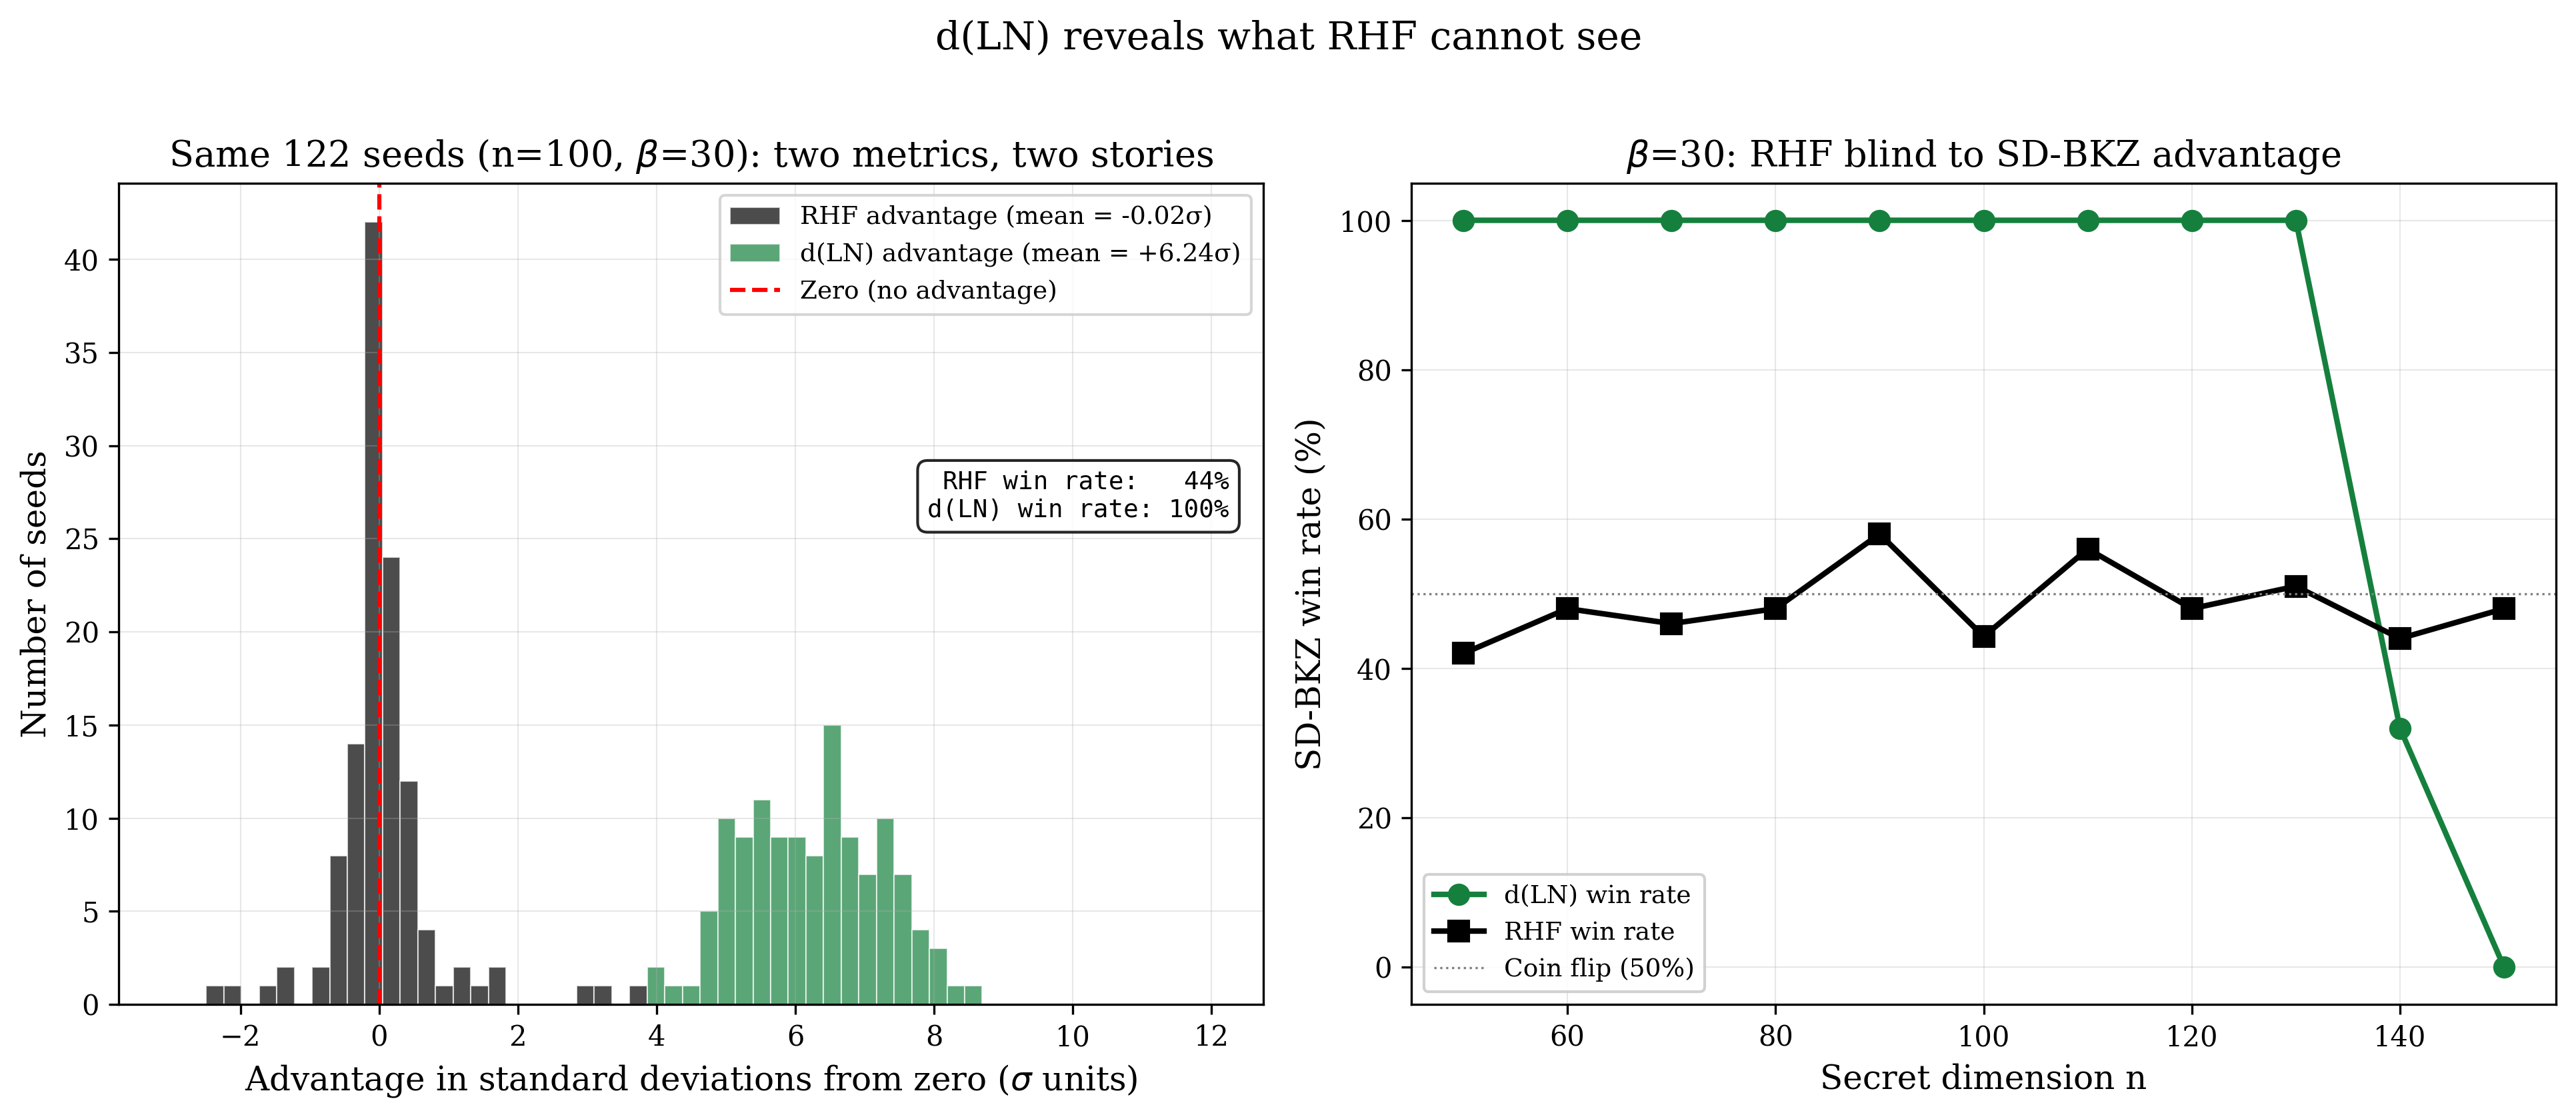
\includegraphics[width=\linewidth]{figs/fig01}
\caption{The same 122 seeds ($n=100$, $\beta=30$) tell opposite stories depending on the metric. Left: $z$-score histograms of the per-seed advantage. RHF (grey) is centred on zero (mean $-0.05\sigma$, coin flip); $d(\mathrm{LN})$ (green) sits $6.24\sigma$ from zero with no overlap (this group; peak effect is $9.6\sigma$ at $n=100$, $\beta=40$). Right: SD-BKZ win rate by dimension for $\beta=30$. $d(\mathrm{LN})$ shows 100\% win rate through $n=130$ before collapsing; RHF fluctuates around 50\% at every dimension, blind to the structural difference.\label{fig:dln-vs-rhf}}
\end{figure}

\paragraph{Statistical rigour.}
At favourable dimensions ($n=50$--$120$), all groups show statistically significant $d(\mathrm{LN})$ advantages for SD-BKZ. Paired $t$-tests reject the null hypothesis of zero mean advantage with $p<10^{-15}$ for 28 of the 33 complete groups; one-sided Wilcoxon signed-rank tests confirm significance without normality assumptions ($p<10^{-10}$ in these groups). Effect sizes range from Cohen's $d=1.31$ ($n=50$, $\beta=40$) to $9.60$ ($n=100$, $\beta=40$). The 95\% confidence intervals on the mean advantage exclude zero in 32 of 33 groups (Table~\ref{tab:stats}). The sole exception is at $n=130$, $\beta=20$, where the CI straddles zero ($[-0.028, +0.034]$, $p=0.85$), the coin-flip transition point. Shapiro--Wilk tests confirm the advantage distributions are consistent with normality ($p>0.05$ in all but one group; the exception at $n=100$, $\beta=20$, $p=0.033$, shows only mild departure that does not affect the paired $t$-test at this sample size). The asymmetry is also quantified precisely: across all groups where BKZ wins any seeds, the mean loss margin is below 0.04 nats, while the mean win margin for SD-BKZ ranges from 0.106 to 1.349 nats.

\begin{table}[tbp]
\centering
\caption{Statistical tests on $d(\mathrm{LN})$ advantage. Effects are large at favourable dimensions and vanish as the advantage declines. All $p$-values are for one-sided tests.\label{tab:stats}}
\small
\begin{tabular}{rrlrll}
\hline
$n$ & $\beta$ & 95\% CI & Cohen's $d$ & $t$-test $p$ & Wilcoxon $p$ \\
\hline
50  & 20 & $[0.262, 0.319]$ & $2.02$  & $<10^{-15}$ & $<10^{-10}$ \\
50  & 30 & $[0.376, 0.433]$ & $2.82$  & $<10^{-15}$ & $<10^{-10}$ \\
50  & 40 & $[0.090, 0.121]$ & $1.31$  & $<10^{-15}$ & $<10^{-10}$ \\
60  & 20 & $[0.278, 0.350]$ & $1.74$  & $<10^{-15}$ & $<10^{-10}$ \\
60  & 30 & $[0.456, 0.524]$ & $2.85$  & $<10^{-15}$ & $<10^{-10}$ \\
60  & 40 & $[0.208, 0.252]$ & $2.06$  & $<10^{-15}$ & $<10^{-10}$ \\
70  & 20 & $[0.380, 0.446]$ & $2.49$  & $<10^{-15}$ & $<10^{-10}$ \\
70  & 30 & $[0.489, 0.559]$ & $2.97$  & $<10^{-15}$ & $<10^{-10}$ \\
70  & 40 & $[0.320, 0.358]$ & $3.55$  & $<10^{-10}$ & $<10^{-10}$ \\
80  & 20 & $[0.439, 0.507]$ & $2.74$  & $<10^{-15}$ & $<10^{-10}$ \\
80  & 30 & $[0.542, 0.618]$ & $3.01$  & $<10^{-15}$ & $<10^{-10}$ \\
80  & 40 & $[0.382, 0.433]$ & $3.13$  & $<10^{-15}$ & $<10^{-10}$ \\
90  & 20 & $[0.444, 0.523]$ & $2.43$  & $<10^{-15}$ & $<10^{-10}$ \\
90  & 30 & $[0.882, 0.962]$ & $4.60$  & $<10^{-15}$ & $<10^{-10}$ \\
90  & 40 & $[0.452, 0.514]$ & $3.04$  & $<10^{-15}$ & $<10^{-10}$ \\
100 & 20 & $[0.328, 0.396]$ & $2.12$  & $<10^{-15}$ & $<10^{-10}$ \\
100 & 30 & $[1.310, 1.387]$ & $6.24$  & $<10^{-15}$ & $<10^{-10}$ \\
100 & 40 & $[1.147, 1.191]$ & $9.60$  & $<10^{-15}$ & $<10^{-10}$ \\
110 & 20 & $[0.203, 0.267]$ & $1.47$  & $<10^{-15}$ & $<10^{-10}$ \\
110 & 30 & $[1.072, 1.151]$ & $5.64$  & $<10^{-15}$ & $<10^{-10}$ \\
110 & 40 & $[1.133, 1.194]$ & $6.82$  & $<10^{-15}$ & $<10^{-10}$ \\
120 & 20 & $[0.063, 0.125]$ & $0.60$  & $3.3\times 10^{-8}$ & $1.4\times 10^{-7}$ \\
120 & 30 & $[0.711, 0.771]$ & $4.97$  & $<10^{-15}$ & $<10^{-10}$ \\
120 & 40 & $[-0.048, -0.008]$ & $-0.28$ & $0.008$ & $0.99$ \\
130 & 20 & $[-0.029, 0.035]$ & $0.02$  & $0.85$ & $0.74$ \\
130 & 30 & $[0.330, 0.374]$ & $3.19$  & $<10^{-15}$ & $<10^{-10}$ \\
130 & 40 & $[-1.352, -1.298]$ & $-8.81$ & $<10^{-15}$ & $1.0$ \\
140 & 20 & $[-0.136, -0.080]$ & $-0.76$ & $1.7\times 10^{-11}$ & $6.2\times 10^{-10}$ \\
140 & 30 & $[-0.053, -0.019]$ & $-0.42$ & $7\times 10^{-5}$ & $1.5\times 10^{-4}$ \\
140 & 40 & $[-1.496, -1.409]$ & $-6.59$ & $<10^{-15}$ & $1.0$ \\
150 & 20 & $[-0.201, -0.145]$ & $-1.21$ & $<10^{-15}$ & $<10^{-10}$ \\
150 & 30 & $[-0.415, -0.374]$ & $-3.88$ & $<10^{-15}$ & $<10^{-10}$ \\
150 & 40 & $[-1.333, -1.253]$ & $-6.30$ & $<10^{-15}$ & $1.0$ \\
\hline
\end{tabular}
\end{table}

\subsection{Outlier Seeds and RHF Fragility}
\label{sec:outliers}

Five groups in Table~\ref{tab:main} (marked $\ast$) show anomalous mean RHF advantages. These are driven by single outlier seeds and vividly illustrate why RHF fails as a quality metric.

At $n=60$, $\beta=20$, one seed (seed 70) produces a pathological SD-BKZ first basis vector with $\mathrm{RHF}=4.67$, approximately $8.5\times$ the group mean of 0.55. This single seed shifts the group's mean RHF advantage to $-0.042$ with standard deviation 0.41, while the remaining 99 seeds show $|\mathrm{RHF\ advantage}|<10^{-7}$. The median RHF advantage for the group is $-6.2\times 10^{-11}$, consistent with all other parameter groups. Similar outlier effects appear at $n=70$ ($\beta=20$: mean RHF $\Delta=+0.70$, $\mathrm{std}=2.18$; $\beta=30$: mean RHF $\Delta=-0.41$, $\mathrm{std}=2.05$) and at $n=80$ ($\beta=30$: mean RHF $\Delta=+0.20$; $\beta=40$: mean RHF $\Delta=+0.29$). The pattern of rare, large RHF outliers driven by single anomalous seeds persists across dimensions.

Crucially, all five outlier seeds still exhibit positive $d(\mathrm{LN})$ advantages---the interior basis structure remains superior despite a degraded first vector. These outlier seeds show anomalously \emph{long} first vectors, which is distinct from the ``head concavity'' phenomenon characterised by Bai, Stehl\'{e} and Wen~\cite{AC:BaiSteWen18}, where BKZ-reduced bases systematically produce \emph{shorter}-than-predicted first vectors. Whether these rare pathological seeds represent an exaggerated or inverted form of head concavity in SD-BKZ warrants further investigation.

The core lesson is structural: a single anomalous shortest vector dominates the RHF scalar while the quality of the remaining $3n$ Gram--Schmidt vectors is ignored. A metric that can be distorted by one vector out of the full $3n+1$-dimensional basis is not a reliable basis for algorithm comparison.

\section{Characterising the SD-BKZ Advantage}
\label{sec:characterising}

\subsection{Asymmetric Effect Size}

The win rate alone understates the result. When SD-BKZ wins (the vast majority of seeds), the advantage is substantial: typically 0.2--0.5 nats. When BKZ wins (the minority), the margin is negligible: below 0.04 nats across all groups. This asymmetry means the $d(\mathrm{LN})$ advantage is not a noisy symmetric effect---it is a one-sided structural improvement.

The effect is most consistent at $\beta=40$, $n=100$, where the standard deviation (0.122) is roughly one-tenth of the mean (1.169), the win rate is 100\%, and Cohen's $d$ reaches 9.60, the highest in the dataset. At $\beta=40$, $n=70$, the ratio is also tight (std 0.096, mean 0.339, $d=3.55$). This suggests the backward pass produces a more deterministic improvement when the SVP oracle is strong.

The weakest group ($n=50$, $\beta=40$, 90\% win rate, Cohen's $d=1.31$) was investigated in detail. The 10 seeds where BKZ achieves lower $d(\mathrm{LN})$ show advantages of $-0.002$ to $-0.082$ nats (mean $-0.039$), approximately $3\times$ smaller in magnitude than the mean winning margin of $+0.122$ nats. The losing seeds are scattered across the seed range with no clustering, show identical initial RHF to winning seeds, and all reached the maximum tour count without stagnating. Crossover analysis reveals that SD-BKZ led BKZ in every losing seed at earlier tours (crossover tours 3--18) before BKZ marginally overtook it by tour 100. This is consistent with under-convergence at the tour limit rather than a genuine BKZ advantage: both algorithms are still slowly improving at tour 100, and the 10 ``losses'' are coin-flip outcomes in the convergence noise.

\begin{figure}[tbp]
\centering
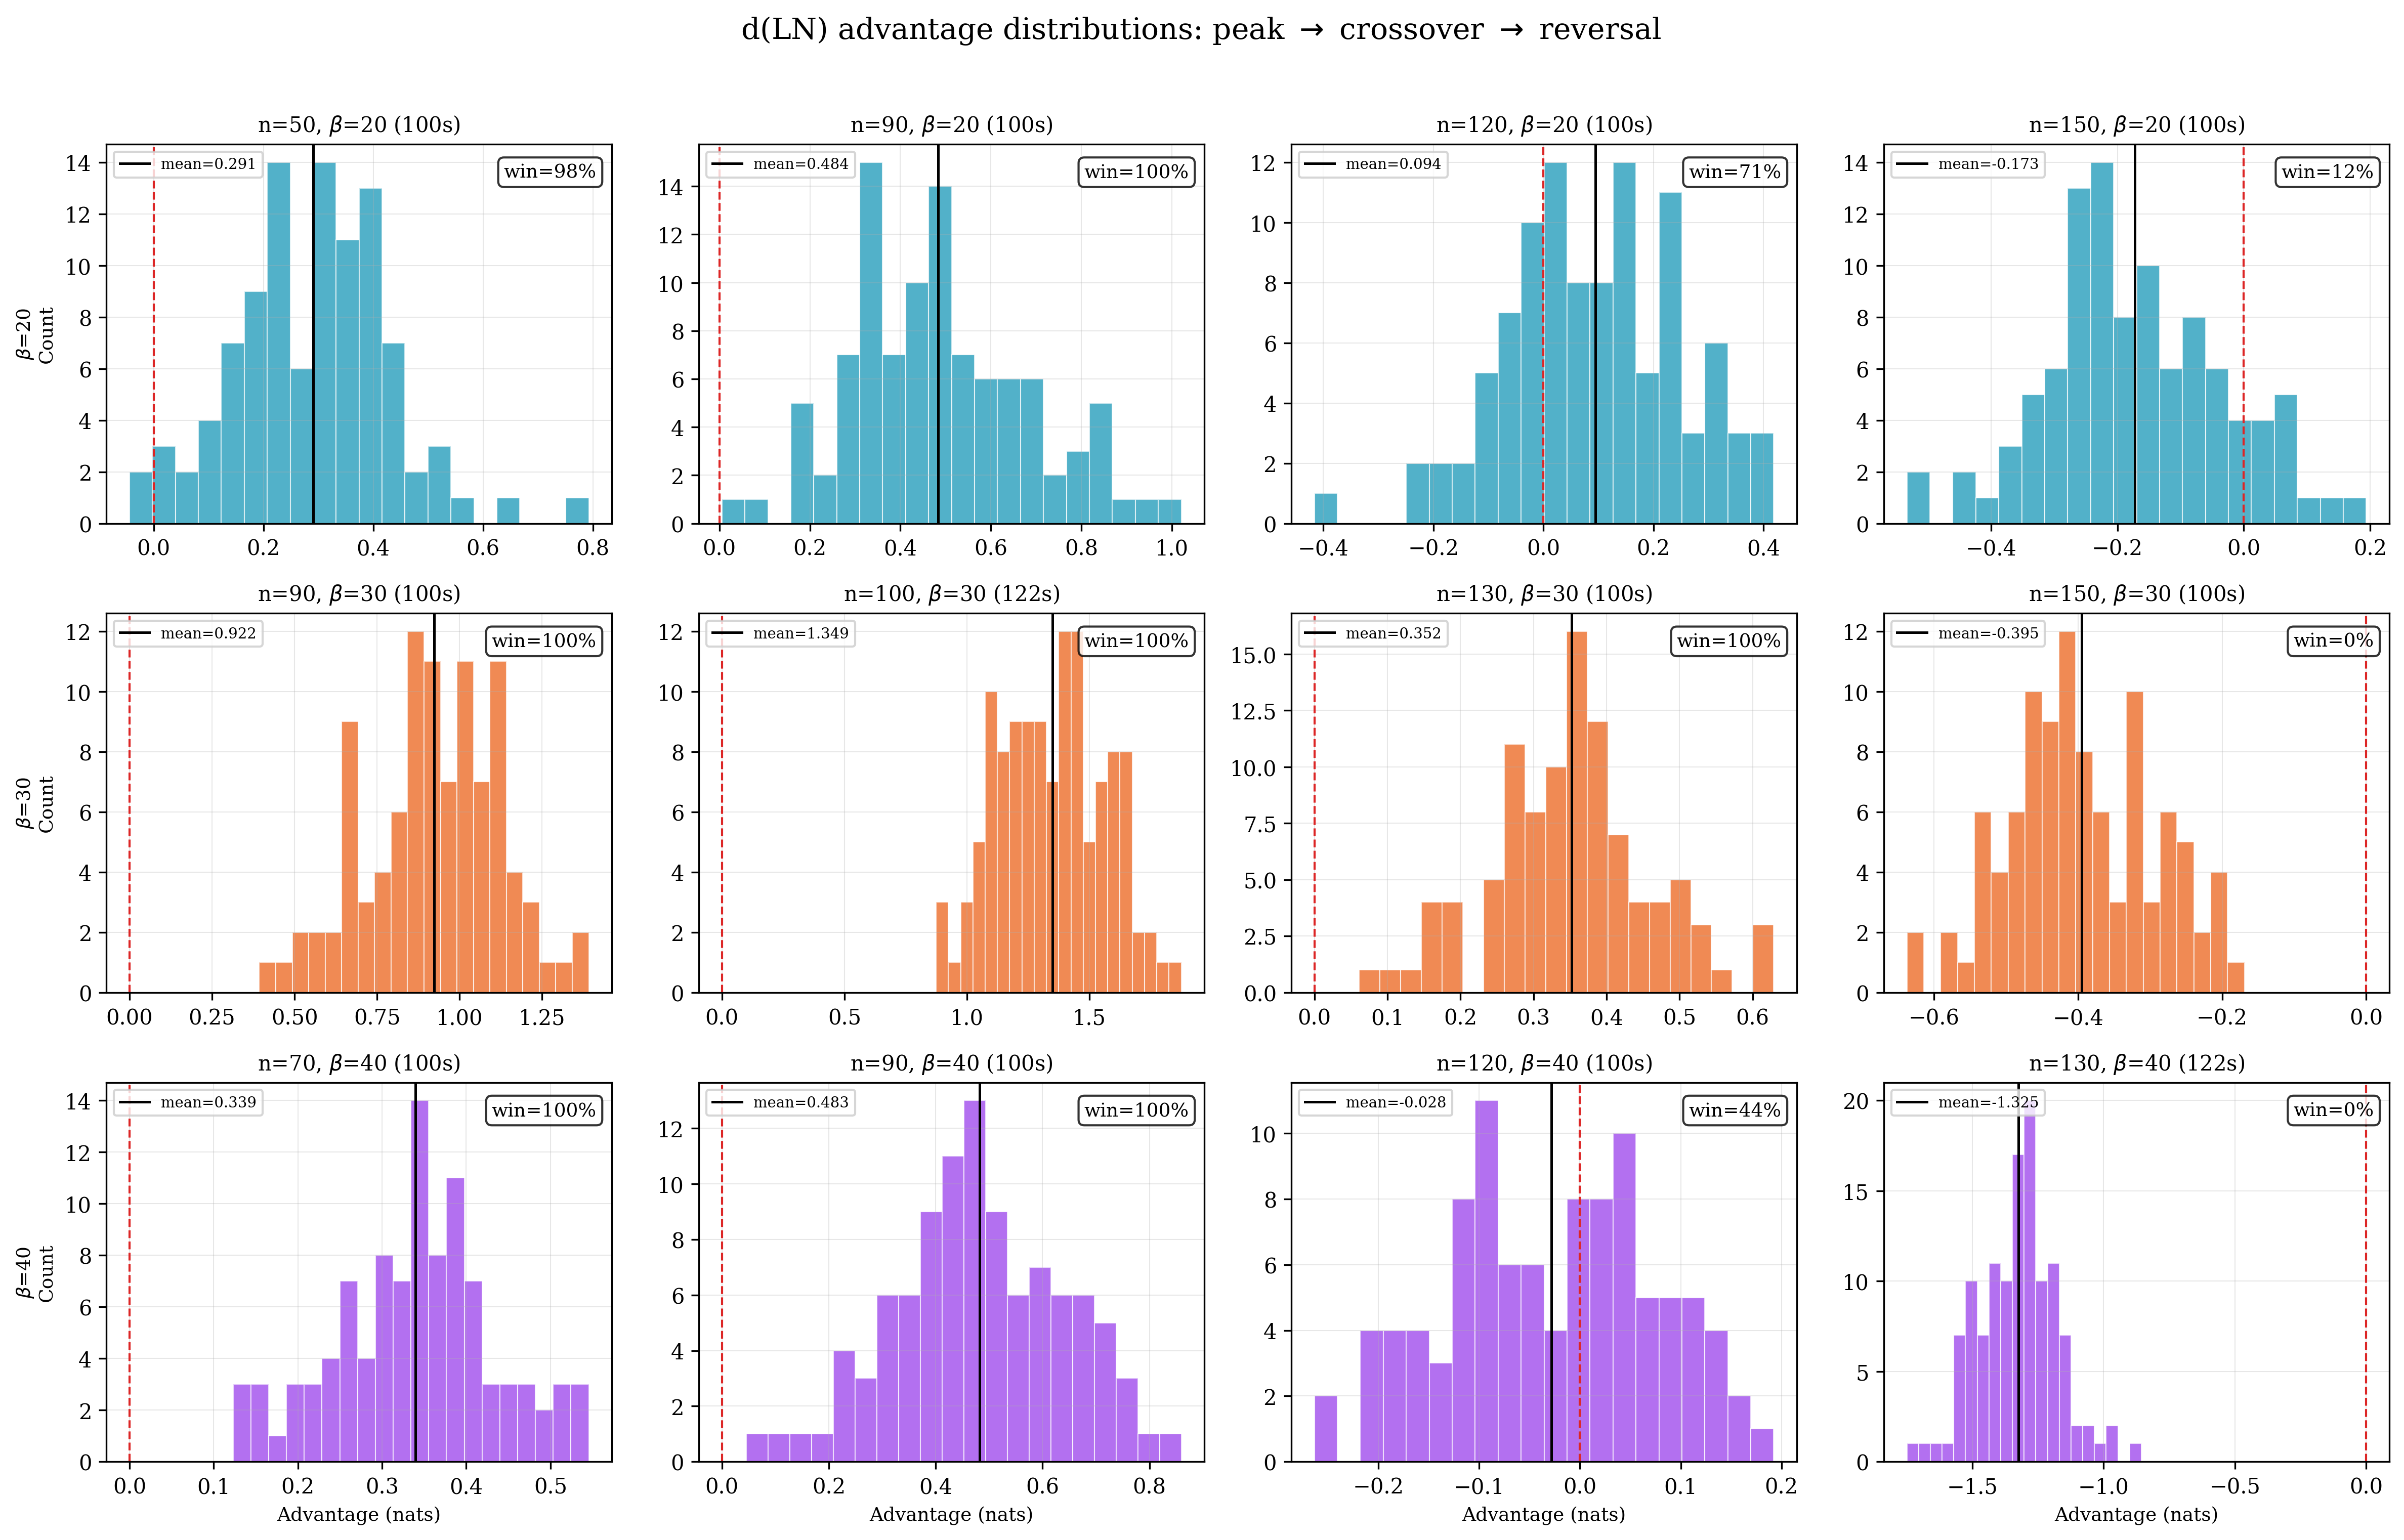
\includegraphics[width=\linewidth]{figs/fig02}
\caption{Per-seed $d(\mathrm{LN})$ advantage distributions showing the full rise, crossover, and reversal pattern for all three block sizes. Each row corresponds to one $\beta$, progressing from peak (left) through crossover to reversal (right). At $\beta=30$, $n=100$ (peak), the entire distribution sits above 0.5 nats with 100\% win rate; by $n=150$, the distribution is entirely negative (0\% win). At $\beta=40$, the reversal is an order of magnitude larger: $n=130$ shows mean $-1.325$ nats with no overlap with zero.\label{fig:histograms}}
\end{figure}

\subsection{Convergence Trajectories}

Neither algorithm converges to the fixed point within the allotted tours: all seeds reach the maximum tour count. However, per-tour $d(\mathrm{LN})$ trajectories reveal that SD-BKZ drops below BKZ early (crossover at tour 3--23 depending on parameters) and maintains its lead throughout. The crossover is fastest at $\beta=40$ (tour 3--6) and slowest at $\beta=20$ (tour 16--23). As dimension increases from $n=50$ to $n=80$, the crossover tour grows slowly with dimension within each $\beta$ group (e.g., median 16$\to$23 at $\beta=20$ from $n=50$ to $n=80$), suggesting the relative convergence speed is primarily a property of the block size.

SD-BKZ exhibits higher per-tour variance in $d(\mathrm{LN})$ than BKZ, but its mean remains consistently lower. This suggests the backward pass introduces more stochasticity per tour while still producing a net improvement. However, per-tour advantage trajectories are non-monotonic: the advantage at any given intermediate tour is not predictive of the final advantage. In individual seeds, the advantage can oscillate from positive to negative and back before settling. This means early-tour $d(\mathrm{LN})$ cannot serve as a cheap signal for which algorithm to commit to---the full tour budget is needed for a reliable comparison.

\begin{figure}[tbp]
\centering

\includegraphics[width=\linewidth]{figs/fig03}
\caption{Per-tour $d(\mathrm{LN})$ trajectories (mean $\pm 1\sigma$ bands, individual seeds in light traces) for $\beta=30$ across four dimensions. (a) $n=70$: SD-BKZ separates early and maintains its lead. (b) $n=100$ (peak): SD-BKZ descends steadily while BKZ diverges upward after tour 30, producing the largest gap in the dataset. (c) $n=130$: the gap narrows; both algorithms converge but SD-BKZ still leads. (d) $n=150$: the inversion is complete; BKZ sits below SD-BKZ throughout the final tours, showing the backward pass becoming counterproductive.\label{fig:trajectories}}
\end{figure}

\subsection{A Capability Difference, Not Just a Speed Difference}
\label{sec:capability}

It is important to distinguish between convergence speed and convergence target. If SD-BKZ merely reached the same fixed point faster, one could achieve the same result by running BKZ for more tours. We tested this directly across 500 seeds in five groups, running BKZ at $3\times$ the standard tour count and comparing against SD-BKZ at $1\times$.

At $\beta=30$, the result is unambiguous: across 400 seeds at $n=50, 60, 70,$ and $80$, BKZ at 210 tours fails to match SD-BKZ at 70 tours in any seed (0/400 gaps closed). The gap does not narrow with extra tours; in fact, it \emph{widens} with dimension: $+0.38$ nats at $n=50$, $+0.50$ at $n=60$, $+0.55$ at $n=70$, $+0.56$ at $n=80$. BKZ has converged by tour 70; tours 71 through 210 produce oscillation around a floor that SD-BKZ sits well below. This is not a speed difference; it is a capability difference. The backward pass reaches basis states that forward-only BKZ cannot access regardless of runtime budget. Note that this comparison is generous to BKZ: each SD-BKZ tour includes a backward pass costing approximately $2.3$--$2.7\times$ a single BKZ tour (Table~\ref{tab:runtime}), so SD-BKZ at 70 tours consumes roughly the same wall-clock time as BKZ at 160--190 tours. At $n=50$, $\beta=30$, the comparison is concrete: SD-BKZ@70 costs 1{,}486 seconds while BKZ@210 costs approximately 1{,}695 seconds. BKZ receives 14\% more compute and still cannot close the gap.

At $\beta=20$, the picture is different. At $n=60$, BKZ at 150 tours ($3\times$ the standard 50) closes 67\% of the gap and wins 26 of 100 seeds. BKZ is still making progress with extra tours at the weaker oracle strength, it is slow but not structurally limited. This $\beta$-dependent split is informative: the capability gap emerges only when the SVP oracle is strong enough ($\beta\geq 30$) for the backward pass to provide structural improvements that the forward pass cannot replicate. At $\beta=20$, the forward pass has not yet exhausted its own convergence capacity, so additional tours can partially compensate for the lack of a backward pass.

A convergence headroom analysis of per-tour trends at the tour limit provides complementary evidence. In high-advantage groups, BKZ's $d(\mathrm{LN})$ trend over the last 5 tours is positive (stalling or diverging: $+0.041$ at $n=100$, $\beta=30$; $+0.027$ at $n=110$, $\beta=20$), while SD-BKZ's trend is smaller ($+0.010$ and $-0.008$ respectively). BKZ is stalling or diverging in its final tours while SD-BKZ either descends ($n=110$) or stalls at roughly one-quarter the rate ($n=100$). The floor fluctuation ratio (SD-BKZ / BKZ per-tour variance) ranges from 1.0 to 1.4 across favourable groups, confirming both algorithms are at comparable convergence states. The reported $d(\mathrm{LN})$ advantages are therefore conservative: additional tours would be expected to widen, not narrow, the gap.

\begin{figure}[tbp]
\centering
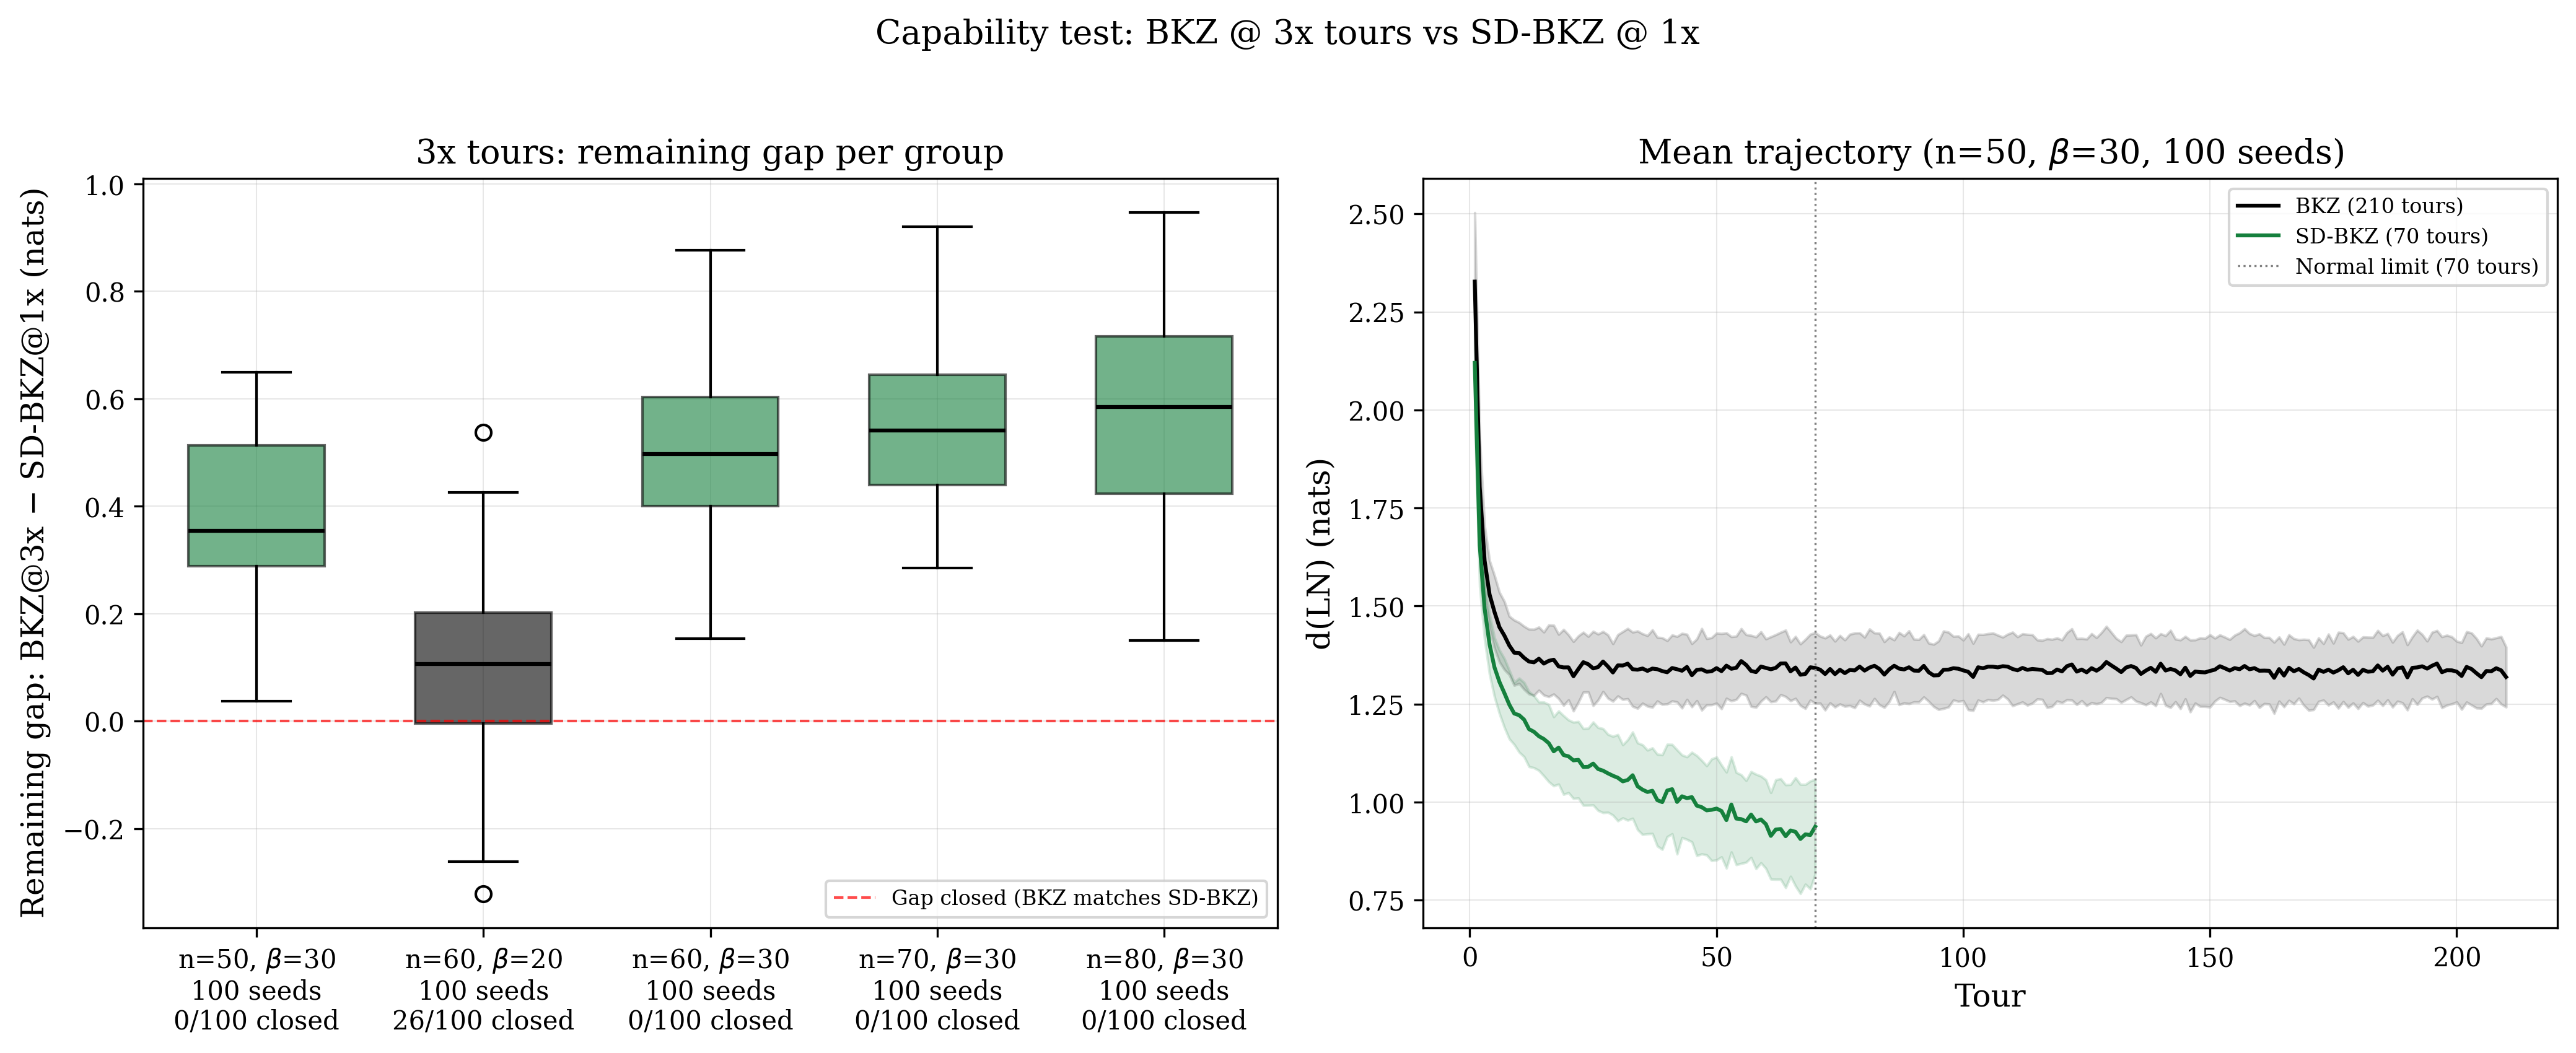
\includegraphics[width=\linewidth]{figs/fig04}
\caption{Capability test: BKZ at $3\times$ tours vs SD-BKZ at $1\times$. Left: remaining gap (BKZ@3x minus SD-BKZ@1x) by group. At $\beta=30$ (green boxes), 0/400 gaps closed across four dimensions and the gap widens with $n$. At $\beta=20$ (grey box), BKZ closes 67\% of the gap and wins 26/100 seeds. Right: mean per-tour trajectories at $n=50$, $\beta=30$ (100 seeds), showing BKZ plateauing after tour 70 while SD-BKZ descends steadily.\label{fig:3xtour}}
\end{figure}

A long-tour convergence test at $n=90$, $\beta=30$ (20 seeds, 500 tours) confirms and extends this finding. BKZ flatlines after tour 70, improving by only $+0.042$ nats over 430 additional tours. SD-BKZ continues descending throughout, gaining $+0.448$ nats over the same interval. The advantage widens from $+0.925$ nats at tour 70 (the standard limit) to $+1.331$ nats at tour 500. BKZ has genuinely stalled; SD-BKZ has not. The $d(\mathrm{LN})$ advantages reported throughout this paper, measured at the standard tour limits, are therefore conservative: longer runs would widen every gap where SD-BKZ leads.

The inverse experiment at the crossover dimension ($n=140$, $\beta=30$, 20 seeds, 500 tours) shows a significant BKZ advantage at this budget: BKZ improves more than SD-BKZ past tour 70 ($+0.122$ vs $+0.099$ nats), widening the gap from $-0.052$ at tour 70 to $-0.075$ at tour 500 ($p=0.002$, 20\% SD-BKZ win rate). At 1000 tours, however, this small deficit becomes statistically undetectable (mean $+0.029$ nats, 95\% CI $[-0.021, +0.079]$, $12/20$; ${\approx}0.21$ power at $n=20$; Section~\ref{sec:limitations}): the $n=140$ reversal is real at the standard and 500-tour budgets but not resolvable at full convergence. The robust high-dimension reversal is at $n=150$, where the deficit deepens monotonically with tour budget.

\begin{figure}[tbp]
\centering
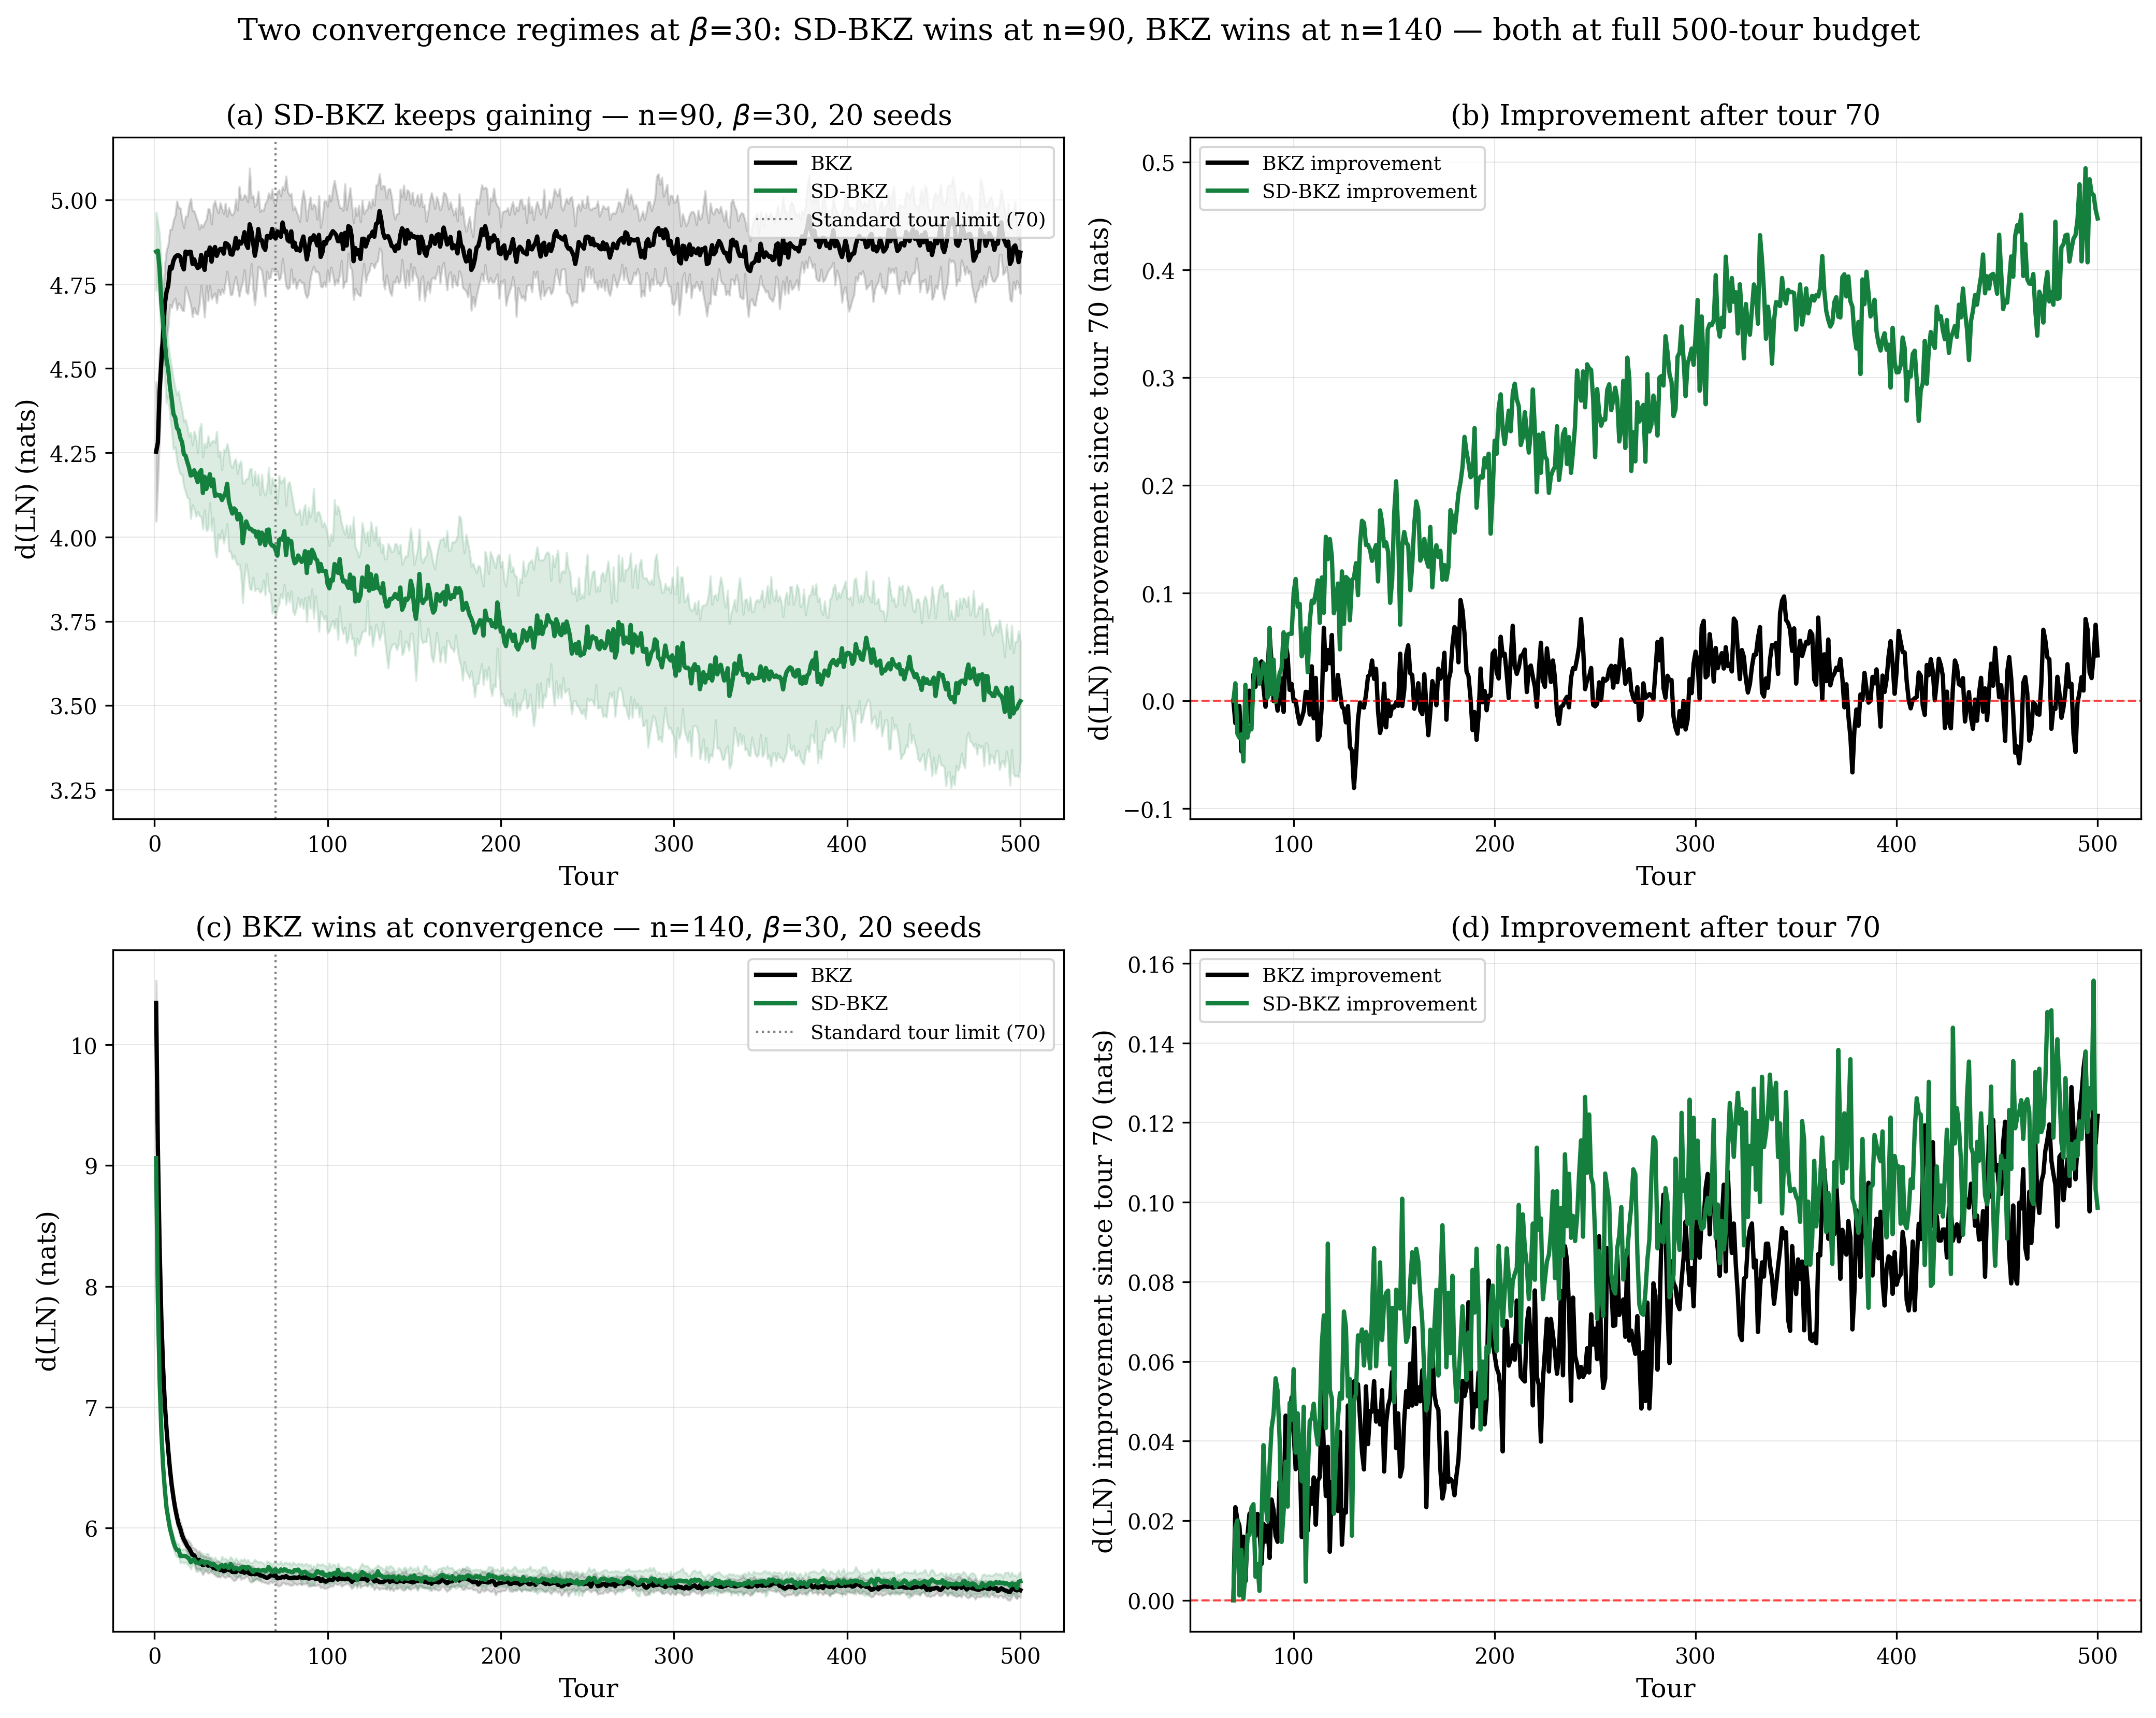
\includegraphics[width=\linewidth]{figs/fig05}
\caption{Two convergence regimes at $\beta=30$ (20 seeds each, 500 tours). Top row ($n=90$): (a) BKZ plateaus after tour ${\sim}70$; SD-BKZ continues descending. (b) Improvement since tour 70: BKZ gains $+0.042$ nats (flat), SD-BKZ gains $+0.448$ nats. The advantage widens from $+0.925$ to $+1.331$. Bottom row ($n=140$, at the crossover): (c) Both algorithms improve slowly past tour 70, with BKZ marginally ahead throughout. (d) BKZ improves $+0.122$ nats vs SD-BKZ $+0.099$ nats; the gap widens slightly to $-0.075$ at $t=500$ (20\% SD-BKZ win); at $t=1000$ this deficit is statistically undetectable ($+0.029$, n.s.; Section~\ref{sec:limitations}).\label{fig:500tour}}
\end{figure}

\subsection{Spatial Decomposition: Where in the Profile Does SD-BKZ Improve?}
\label{sec:spatial}

To understand \emph{where} in the basis SD-BKZ's advantage concentrates, we decompose the $d(\mathrm{LN})$ improvement by position in the Rankin profile. For each seed, we compute the per-position distance to the fixed point for both algorithms ($|R_k - R^*_k|$ for BKZ and SD-BKZ), then measure where SD-BKZ is closer. We partition the profile into three equal segments: head (first third of the active block indices), middle, and tail.

\begin{table}[tbp]
\centering
\caption{Profile-position decomposition of the $d(\mathrm{LN})$ advantage. The middle third dominates across the $n=50$--$110$ favourable regime (21/21 groups); beyond the peak dimension the decomposition flips as described in Figure~\ref{fig:spatial}. Representative subset ($n=50$--$70$); full decomposition for all 33 groups in supplementary JSON (\texttt{results/profile\_decomposition.json}).\label{tab:spatial}}
\small
\begin{tabular}{rrrrrrr}
\hline
$n$ & $\beta$ & Seeds & Head \% & Mid \% & Tail \% & Mid win rate \\
\hline
50 & 20 & 100 & 21\% & 44\% & 35\% & 97\% \\
50 & 30 & 100 & 21\% & 46\% & 33\% & 100\% \\
50 & 40 & 100 & 7\%  & 82\% & 11\% & 91\% \\
60 & 20 & 100 & 22\% & 44\% & 34\% & 94\% \\
60 & 30 & 100 & 19\% & 45\% & 36\% & 100\% \\
60 & 40 & 100 & 25\% & 55\% & 20\% & 96\% \\
70 & 20 & 100 & 20\% & 45\% & 35\% & 98\% \\
70 & 30 & 100 & 18\% & 45\% & 37\% & 100\% \\
70 & 40 & 100 & 25\% & 53\% & 22\% & 100\% \\
\hline
\end{tabular}
\end{table}

The result is unambiguous: the middle third of the Rankin profile accounts for 44--82\% of the total $d(\mathrm{LN})$ improvement in the $n=50$--$70$ subset shown. At $\beta=40$, the concentration is most extreme---at $n=50$, 82\% of the improvement comes from the middle, with head (7\%) and tail (11\%) nearly negligible. The middle-region win rate is 91--100\% across all favourable groups.

This contradicts the na\"{\i}ve expectation that the backward pass primarily improves the ``tail'' of the basis. Standard BKZ sweeps forward, optimising from the head; the middle of the profile is the region the forward pass reaches last and optimises least effectively. SD-BKZ's backward pass (equivalently, a forward pass on the reversed dual basis) works from the opposite direction, reaching the middle from below. The middle is therefore the region where the two passes overlap most productively---it receives optimisation pressure from both directions in SD-BKZ, but only from one direction in standard BKZ.

The $\beta$ dependence is also informative: at $\beta=40$, the SVP oracle is strong enough that the forward pass already handles the head and tail adequately; the residual improvement available is concentrated in the middle. At $\beta=20$, the oracle is weaker everywhere, so the improvement is more diffuse (21/44/35\% head/mid/tail).

\begin{figure}[tbp]
\centering

\includegraphics[width=\linewidth]{figs/fig06}
\caption{Mean $d(\mathrm{LN})$ improvement by profile region (head, middle, tail) across all groups, faceted by block size. At $\beta=20$ (top), the middle dominates through $n=100$, but the tail flips negative from $n=110$ onward as the backward pass overcorrects the tail positions. At $\beta=30$ (middle), the middle peaks at $n=100$--$110$ ($+1.9$ to $+2.0$ nats) before flipping strongly negative at $n=140/150$, indicating BKZ wins the middle at high dimensions. At $\beta=40$ (bottom), the cliff is visible: all three regions improve dramatically at $n=100$--$110$ before collapsing below zero at $n\geq 120$, with every region simultaneously flipping sign.\label{fig:spatial}}
\end{figure}

At higher dimensions where the advantage is collapsing, the spatial distribution shifts dramatically. At $n=130$, $\beta=20$ (mean advantage 0.003, 54\% win), the residual improvement is almost entirely in the head of the profile (Figure~\ref{fig:spatial}). At this low $\beta/n$ ratio (0.15), the block size is too small relative to the lattice dimension for the dual-direction sweep to provide meaningful coverage of the middle region. The decline at $\beta\geq 30$ has a different character: per-position analysis (Section~\ref{sec:peakmigration}) shows that the backward pass retains its reach into the middle but increasingly overcorrects the tail, with the resulting negative dip eventually overwhelming the positive contribution.

The GSO log-norm profiles (Figure~\ref{fig:gso}) reveal a complementary structural difference: at $n\geq 130$, BKZ exhibits a sharp downward hook at the tail of the basis (the last few Gram--Schmidt log-norms curve below the Li--Nguyen prediction because BKZ cannot apply a full $\beta$-block when fewer than $\beta$ vectors remain). SD-BKZ produces a smooth taper into the same final region, visually eliminating the hook. However, per-position analysis against the Rankin fixed point $R^*$ reveals a subtlety: at a small number of tail positions (e.g., positions 91--94 at $n=100$, $\beta=30$), BKZ is actually \emph{closer} to $R^*$ than SD-BKZ. The backward pass overcorrects these positions, pushing them further below the fixed point than BKZ's hook does. At position~93, BKZ is within 0.2~nats of $R^*$ in 97\% of seeds, while SD-BKZ undershoots by 0.78~nats. The two algorithms thus produce different tail geometries, neither strictly closer to $R^*$ at every position. This tail overcorrection is small at favourable dimensions but grows with $n$, and is the primary mechanism behind the advantage decline described in Section~\ref{sec:blocksize} (see Figure~\ref{fig:perpos} for the full per-position landscape across all 33 groups).

\begin{figure}[tbp]
\centering

\includegraphics[width=\linewidth]{figs/fig07}
\caption{Mean Rankin profiles for BKZ (black) and SD-BKZ (green) at $\beta=30$ across four dimensions. SD-BKZ sits consistently below BKZ in the middle region (lower = closer to the fixed point), confirming the spatial decomposition finding. The gap is largest at $n=100$ (b) and narrowest at $n=150$ (d), where both profiles nearly overlap, consistent with the vanishing advantage.\label{fig:profiles}}
\end{figure}

\begin{figure}[tbp]
\centering

\includegraphics[width=\linewidth]{figs/fig08}
\caption{Mean Gram--Schmidt log-norm profiles ($\log\|b^*_i\|$) for BKZ (black) and SD-BKZ (green) with theoretical predictions: GSA (red dotted) and Li--Nguyen fixed point (orange dashed). At $n=70$ (a), both algorithms track the LN prediction closely. At $n=100$ (b), SD-BKZ follows the LN prediction more faithfully through the middle region while BKZ deviates. At $n=130$--$150$ (c,d), BKZ exhibits a pronounced tail hook (GS log-norms dropping below zero in a sharp downward curve), while SD-BKZ produces a smooth taper into the same final region. The backward pass reshapes the tail geometry rather than simply eliminating the hook; per-position analysis shows BKZ is closer to $R^*$ at a small number of tail positions where SD-BKZ overcorrects (Section~\ref{sec:spatial}). The head concavity phenomenon~\cite{AC:BaiSteWen18} is visible at all dimensions.\label{fig:gso}}
\end{figure}

\section{Block Size and Dimension Dependence}
\label{sec:blocksize}

\subsection{Non-Monotonic Block Size Relationship}

The advantage peaks at $\beta=30$ at most measured dimensions, but the relationship is dimension-dependent. At $n=110$, $\beta=40$ overtakes $\beta=30$ ($+1.163$ vs $+1.112$; 122 and 100 seeds respectively) before collapsing dramatically (Table~\ref{tab:beta-n-matrix}, Figure~\ref{fig:dim-scaling}).

\begin{table}[tbp]
\centering
\caption{$d(\mathrm{LN})$ advantage by block size and dimension. Bold indicates the peak for each block size. 100 seeds per group (122 for four variance-filled groups; see Table 3).\label{tab:beta-n-matrix}}
\small
\setlength{\tabcolsep}{4pt}
\begin{tabular}{rrrrrrrrrrrr}
\hline
$\beta$ & $n{=}50$ & $60$ & $70$ & $80$ & $90$ & $100$ & $110$ & $120$ & $130$ & $140$ & $150$ \\
\hline
20 & 0.291 & 0.314 & 0.413 & 0.473 & $\mathbf{0.484}$ & 0.362 & 0.235 & 0.094 & 0.003 & $-0.108$ & $-0.173$ \\
30 & 0.405 & 0.490 & 0.524 & 0.580 & 0.922 & $\mathbf{1.349}$ & 1.112 & 0.741 & 0.352 & $-0.036$ & $-0.395$ \\
40 & 0.106 & 0.230 & 0.339 & 0.408 & 0.483 & 1.169 & $\mathbf{1.163}$ & $-0.028$ & $-1.325$ & $-1.452$ & $-1.293$ \\
\hline
\end{tabular}
\end{table}

\begin{figure}[tbp]
\centering
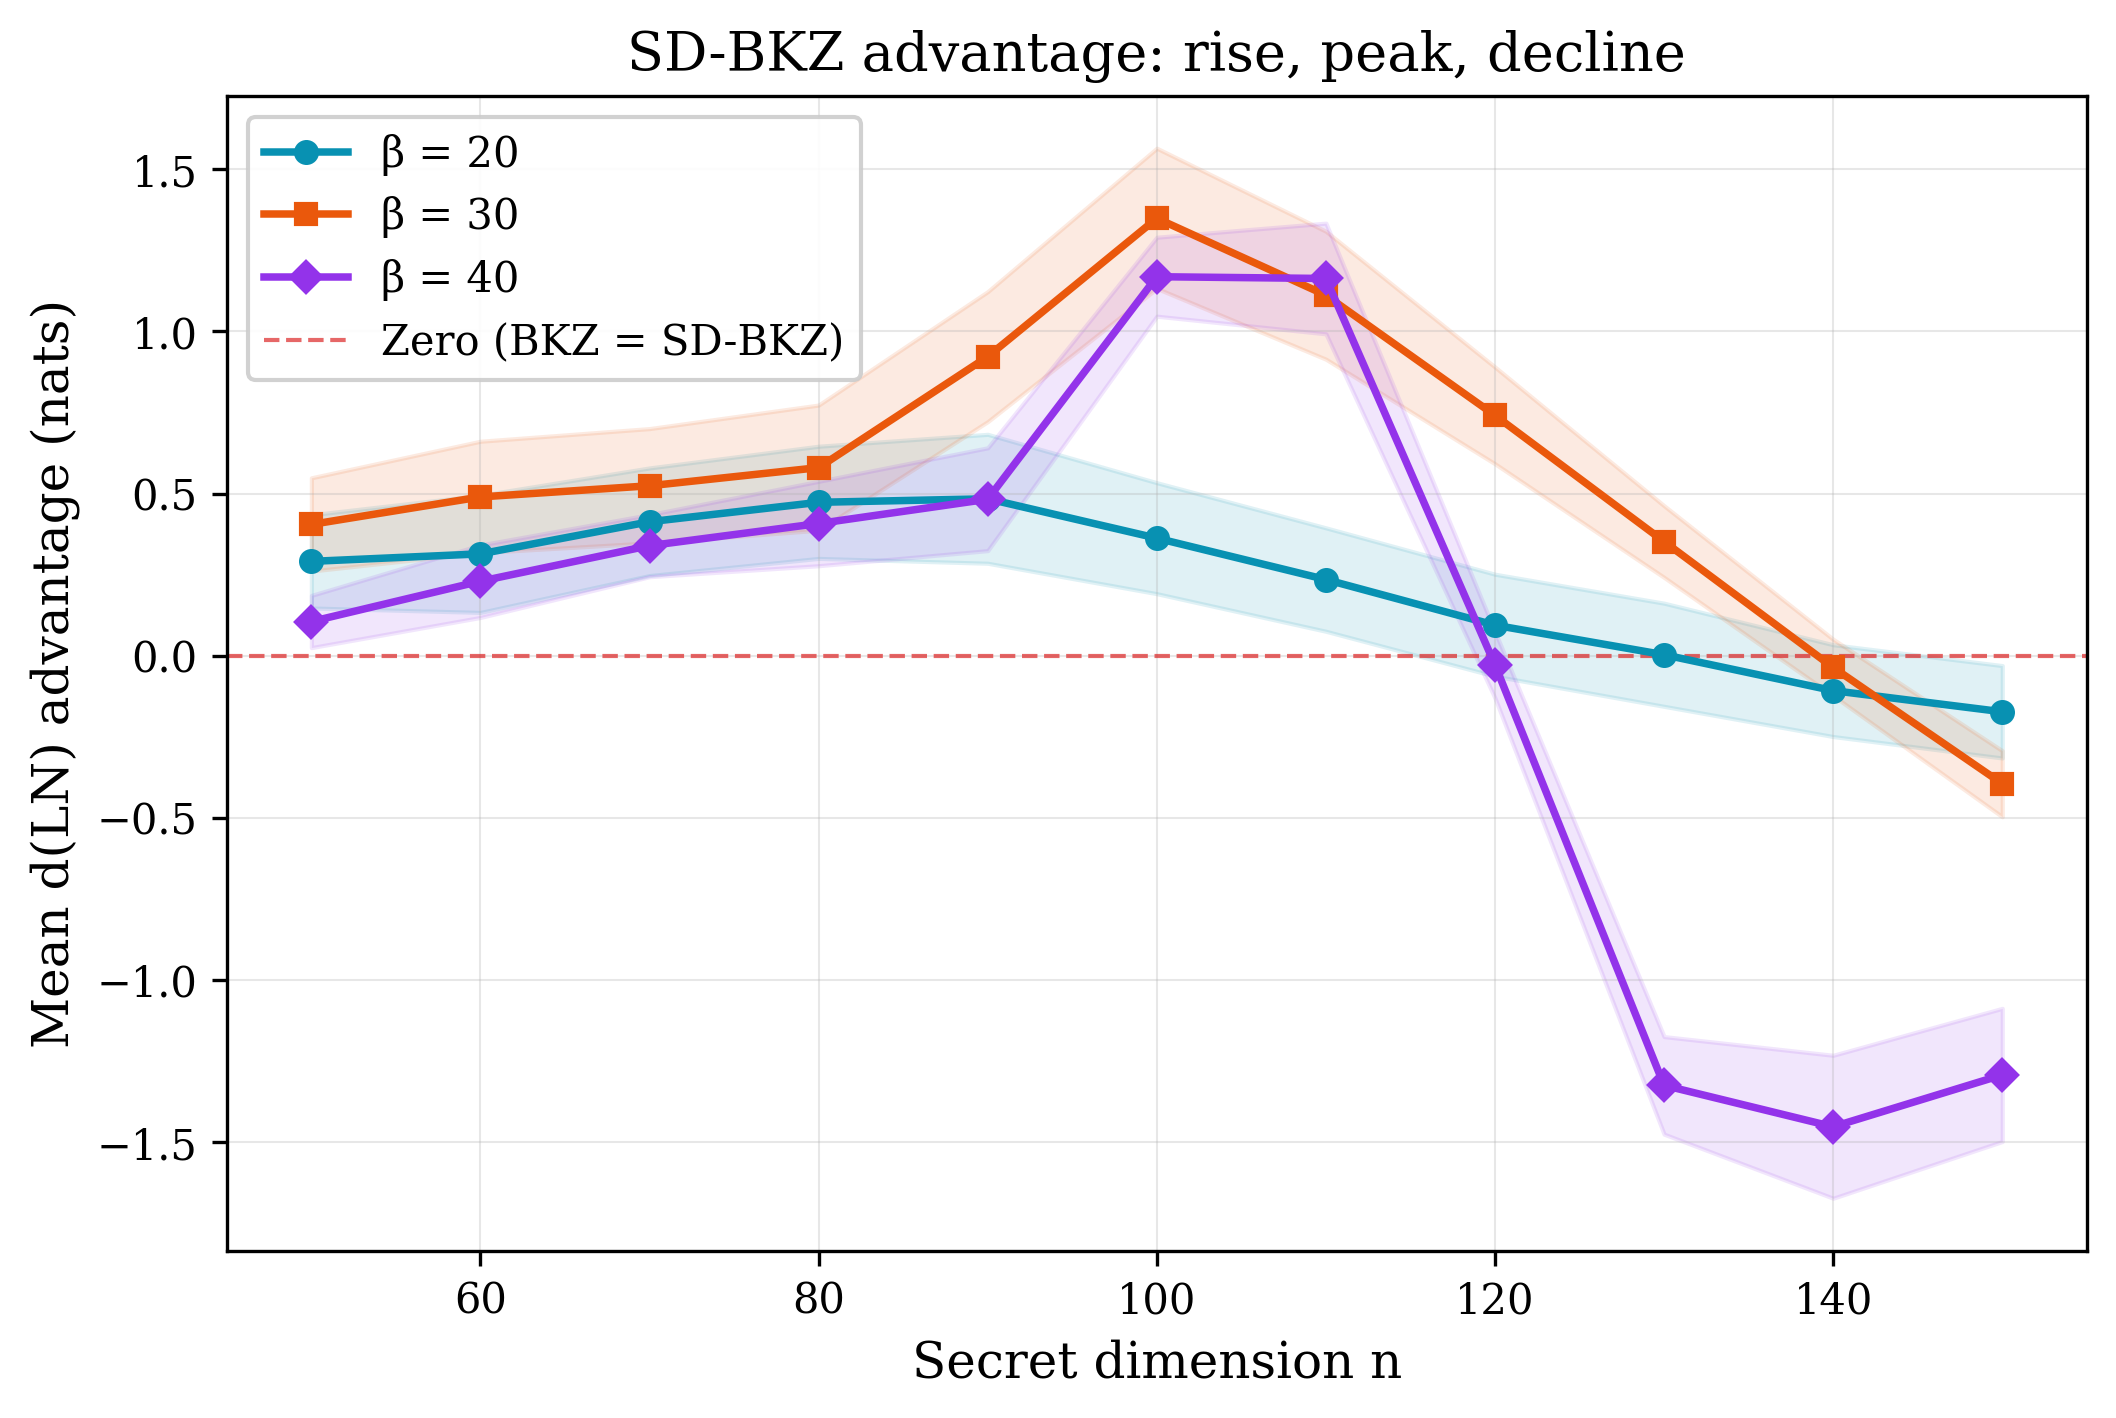
\includegraphics[width=\linewidth]{figs/fig09}
\caption{Mean $d(\mathrm{LN})$ advantage ($\pm 1\sigma$) as a function of secret dimension $n$ for each block size. The peak dimension is block-size-dependent: $\beta=20$ peaks at $n=90$, $\beta=30$ at $n=100$, and $\beta=40$ at $n=110$. All three block sizes decline into negative territory. The $\beta=40$ cliff ($n=110$ to $n=130$) is the steepest decline in the dataset: a swing of 2.5 nats in two dimension steps.\label{fig:dim-scaling}}
\end{figure}

At $n=50$, the ratio of $\beta=30$ advantage to $\beta=40$ advantage is $3.8{:}1$. At $n=70$, this ratio has narrowed to $1.5{:}1$, and at $n=80$ it is $1.4{:}1$. The $\beta=40$ advantage more than tripled from $n=50$ to $n=70$ ($+222\%$) and continued growing to 0.408 at $n=80$ ($+19\%$). At $n=90$, $\beta=30$ undergoes a dramatic acceleration: the advantage jumps from 0.580 to 0.922 nats ($+59\%$), the largest single-step increase in the completed dataset. This is followed by a decline to 0.741 at $n=120$ and 0.352 at $n=130$. The $\beta=20$ advantage follows a similar pattern, peaking at $n=90$ (0.484) before declining through 0.362 ($n=100$), 0.094 ($n=120$), 0.003 ($n=130$), and $-0.108$ ($n=140$, where BKZ actively wins). The peak dimension is block-size-dependent: $\beta=20$ peaks at $n=90$, while $\beta=30$ peaks at $n=100$ (Section~\ref{sec:dim-scaling}).

Standard BKZ sweeps forward through the basis, optimising from the head. The middle portion of the Gram--Schmidt profile is the last region the forward pass reaches effectively. SD-BKZ adds a backward pass (equivalently, a forward pass on the reversed dual), which works the basis from the opposite direction. As our profile decomposition confirms (Section~\ref{sec:spatial}), the middle of the Rankin profile---not the tail---is where SD-BKZ's improvement concentrates. As lattice dimension grows, this middle region expands, and a larger block size allows each pass to reach further into it. This dimension-dependent interaction has never been empirically measured. The standard metric (RHF) is blind to interior profile improvements, and the SD-BKZ empirical literature has been frozen at 10 instances since 2016. Testing at intermediate block sizes ($\beta\in\{25, 35\}$) would help characterise the transition more precisely.

\subsection{Dimension Scaling}
\label{sec:dim-scaling}

\begin{table}[tbp]
\centering
\caption{Growth rate of $d(\mathrm{LN})$ advantage between dimensions.\label{tab:growth}}
\small
\begin{tabular}{rrrrrrrl}
\hline
$\beta$ & $50{\to}60$ & $60{\to}70$ & $70{\to}80$ & $80{\to}90$ & $90{\to}100$ & $100{\to}110$ & Character \\
\hline
20 & $+8\%$   & $+32\%$ & $+15\%$ & $+2\%$   & $-25\%$  & $-35\%$ & Peak $n{=}90$, collapsing \\
30 & $+21\%$  & $+7\%$  & $+11\%$ & $+59\%$  & $+46\%$  & $-17\%$ & Peak $n{=}100$, declining \\
40 & $+117\%$ & $+48\%$ & $+20\%$ & $+18\%$  & $+144\%$ & $-2\%$  & Peak $n{=}110$, cliff \\
\hline
\end{tabular}
\end{table}

At $\beta=30$, the full trajectory is: $0.405 \to 0.490 \to 0.524 \to 0.580 \to 0.922 \to 1.349 \to 1.112 \to 0.741 \to 0.352 \to -0.036 \to -0.395$ nats from $n=50$ through $n=150$, peaking at $n=100$ ($+46\%$ from $n=90$) then declining sharply. At $\beta=20$, the trajectory is: $0.291 \to 0.314 \to 0.413 \to 0.473 \to 0.484 \to 0.362 \to 0.235 \to 0.094 \to 0.003 \to -0.108 \to -0.173$, peaking at $n=90$ before collapsing. At $\beta=40$, the advantage rises from 0.106 ($n=50$) through 0.483 ($n=90$) and 1.169 ($n=100$, 122 seeds) to a confirmed peak at $n=110$ ($+1.163$, 122 seeds, overtaking $\beta=30$), then collapses catastrophically: $-0.028$ at $n=120$, $-1.325$ at $n=130$, $-1.452$ at $n=140$, $-1.293$ at $n=150$ (0\% win). The peak dimension migrates upward with block size: $\beta=20$ at $n=90$, $\beta=30$ at $n=100$, $\beta=40$ at $n=110$.

The variance behaviour also differs by block size. At $\beta=40$, $n=70$, the standard deviation is 0.096, roughly one-quarter of the mean. At $\beta=30$, the standard deviation remains stable at 0.10--0.22 across dimensions. At $\beta=40$, $n=130$, the standard deviation is 0.150 against a mean of $-1.325$, giving Cohen's $d\approx -9$: BKZ wins every seed (0/122) by a large margin. The backward pass is not just ineffective at high dimensions; it is deterministically harmful.

\subsection{Block-Size-Dependent Peak Migration and the $\beta=40$ Cliff}
\label{sec:peakmigration}

The SD-BKZ advantage does not grow monotonically with dimension, and the peak dimension is not universal. At $\beta=20$, the advantage peaks at $n=90$ (0.484 nats), then declines smoothly through 0.235 ($n=110$) and 0.094 ($n=120$) to a coin-flip region at $n=130$ (0.003 nats, 54\% win), and into active BKZ superiority at $n=140$ ($-0.108$ nats, 22\% win) and $n=150$ ($-0.173$ nats, 12\% win). At $\beta=30$, the peak migrates to $n=100$ (1.349 nats, the largest mean advantage in the dataset), followed by decline to 1.112 ($n=110$) and 0.741 ($n=120$), crossing zero near $n=140$ ($-0.036$, 100 seeds, 32\% win) and reaching $-0.395$ at $n=150$ (0\% win rate, 100 seeds).

The $\beta=40$ trajectory reveals the most dramatic behaviour in the dataset. The advantage rises steadily from $+0.106$ at $n=50$ through $+0.483$ at $n=90$, reaches $+1.163$ at $n=110$ (122 seeds, overtaking $\beta=30$), then falls off a cliff: $-0.028$ at $n=120$ (44\% win), $-1.325$ at $n=130$ (0\% win), $-1.452$ at $n=140$ (0\% win), $-1.293$ at $n=150$ (0\% win). This is a swing of 2.5 nats in two dimension steps ($n=110$ to $n=130$), an order of magnitude steeper than the $\beta=30$ decline (1.75 nats over five steps) or the $\beta=20$ decline (0.66 nats over six steps). The inversion severity scales with block size: larger $\beta$ produces both higher peaks and steeper collapses. The slight recovery from $-1.452$ at $n=140$ to $-1.293$ at $n=150$ suggests the decline may not be monotonic beyond the cliff.

\begin{figure}[tbp]
\centering

\includegraphics[width=\linewidth]{figs/fig10}
\caption{Absolute $d(\mathrm{LN})$ (distance to Li--Nguyen fixed point) for BKZ and SD-BKZ across dimensions, separated by block size. At $\beta=20$, both algorithms are far from the fixed point (${\sim}15$ nats at $n=120$) and nearly indistinguishable. At $\beta=30$, SD-BKZ is consistently closer through $n=130$, with the gap largest at $n=100$. At $\beta=40$, the curves cross at $n=130$, where SD-BKZ becomes further from the fixed point than BKZ. The $\beta=40$ inversion at $n=150$ (SD-BKZ ${\sim}8.4$ vs BKZ ${\sim}6.8$) shows the backward pass actively pushing the basis away from the fixed point at high dimensions.\label{fig:abs-dln}}
\end{figure}

\begin{table}[tbp]
\centering
\caption{Dimension scaling at and beyond the peak. The peak dimension migrates upward with block size.\label{tab:peak}}
\small
\begin{tabular}{rrrrrrr}
\hline
$n$ & $\beta$ & Seeds & $\beta/n$ & Mean adv. & Std & Win rate \\
\hline
90  & 20 & 100 & 0.22 & 0.484   & 0.198 & 100\% \\
90  & 30 & 100 & 0.33 & 0.922   & 0.199 & 100\% \\
90  & 40 & 100 & 0.44 & 0.483   & 0.159 & 100\% \\
100 & 20 & 100 & 0.20 & 0.362   & 0.171 & 99\%  \\
100 & 30 & 122 & 0.30 & 1.349   & 0.216 & 100\% \\
100 & 40 & 122 & 0.40 & 1.169   & 0.122 & 100\% \\
110 & 20 & 100 & 0.18 & 0.235   & 0.160 & 92\%  \\
110 & 30 & 100 & 0.27 & 1.112   & 0.197 & 100\% \\
110 & 40 & 122 & 0.36 & 1.163   & 0.171 & 100\% \\
120 & 20 & 100 & 0.17 & 0.094   & 0.157 & 71\%  \\
120 & 30 & 100 & 0.25 & 0.741   & 0.149 & 100\% \\
120 & 40 & 100 & 0.33 & $-0.028$ & 0.102 & 44\%  \\
130 & 20 & 100 & 0.15 & 0.003   & 0.159 & 54\%  \\
130 & 30 & 100 & 0.23 & 0.352   & 0.111 & 100\% \\
130 & 40 & 122 & 0.31 & $-1.325$ & 0.150 & 0\%   \\
140 & 20 & 100 & 0.14 & $-0.108$ & 0.142 & 22\%  \\
140 & 30 & 100 & 0.21 & $-0.036$ & 0.087 & 32\%  \\
140 & 40 & 100 & 0.29 & $-1.452$ & 0.220 & 0\%   \\
150 & 20 & 100 & 0.13 & $-0.173$ & 0.142 & 12\%  \\
150 & 30 & 100 & 0.20 & $-0.395$ & 0.102 & 0\%   \\
150 & 40 & 100 & 0.27 & $-1.293$ & 0.205 & 0\%   \\
\hline
\end{tabular}
\end{table}

The $\beta/n$ ratio alone does not explain this pattern. At $n=110$, $\beta=40$ ($\beta/n=0.36$) shows the highest advantage of any $\beta=40$ group ($+1.163$, 122 seeds), but just two dimension steps later at $n=130$ ($\beta/n=0.31$) it has collapsed to $-1.325$ (0\% win, 122 seeds). Meanwhile, $\beta=30$ at $n=130$ ($\beta/n=0.23$) remains positive ($+0.352$, 100\% win). The $\beta=40$ cliff is not predicted by $\beta/n$ and is an order of magnitude steeper than the $\beta=30$ decline.

\begin{figure}[tbp]
\centering

\includegraphics[width=\linewidth]{figs/fig11}
\caption{Mean $d(\mathrm{LN})$ advantage vs $\beta/n$ ratio for all groups, coloured by block size. Points below the dashed red line indicate BKZ superiority. The shaded region ($\beta/n<0.20$) marks the ``collapse zone'' for $\beta=20$. The $\beta=40$ cliff is clearly visible: $n=110$ ($+1.16$ at $\beta/n=0.36$) drops to $n=130$ ($-1.32$ at $\beta/n=0.31$) and $n=140$ ($-1.45$ at $\beta/n=0.29$), despite $\beta/n$ ratios that remain above 0.20. 100 seeds per group (122 for four variance-filled groups; see Table 3). The $\beta/n$ ratio alone does not govern backward pass effectiveness.\label{fig:beta-n-scatter}}
\end{figure}

The $\beta=40$ cliff complicates the convergence depth explanation. If the negative advantage at $n=120$--$150$ were purely due to insufficient convergence, we would not expect $\beta=40$ to \emph{overtake} $\beta=30$ at $n=110$ ($+1.163$ vs $+1.112$) before collapsing. The backward pass is clearly effective at $n=110$ with the same tour budget that produces catastrophic failure two dimension steps later. This suggests the cliff is a structural breakdown, not an artifact of under-convergence: there is a dimension threshold beyond which the backward pass on a 40-dimensional sublattice actively degrades the basis rather than improving it. Whether this threshold can be shifted by increasing the tour count remains an open question; a $3\times$ tour test at $\beta=40$ (analogous to Section~\ref{sec:capability}) would be informative but is computationally prohibitive at these dimensions (a single seed at $n=130$, $\beta=40$, 300 tours requires approximately 25{,}000 seconds based on Table~\ref{tab:runtime} extrapolation).

SD-BKZ effectiveness depends on at least three interacting factors: block size, lattice dimension, and convergence depth (tour count relative to per-tour cost). The backward pass is beneficial when all three are in a favourable regime. The $\beta=40$ cliff demonstrates that larger block sizes amplify both the peak advantage and the severity of the collapse, suggesting a phase-transition-like boundary in the parameter space.

A per-position decomposition of the Rankin profile reveals that the decline mechanism differs by block size (Figure~\ref{fig:perpos}). At $\beta\in\{20,30\}$, the peak positional advantage (the best single position where SD-BKZ is closest to $R^*$) remains remarkably stable as dimension grows: at $\beta=30$, the peak is $+0.70$~nats at $n=50$ and still $+1.10$~nats at $n=150$ (the collapse dimension). What drives the mean advantage negative is a growing \emph{overcorrection dip} at the tail, where SD-BKZ pushes positions further below $R^*$ than BKZ does. The dip grows from $-0.26$~nats at $n=50$ to $-2.28$ at $n=150$, eventually overwhelming the stable peak. The backward pass does not lose its beneficial reach into the middle; it loses precision at the tail boundary, and the resulting overshoot scales faster than the headline advantage. At $\beta=40$, the mechanism is qualitatively different: both the peak \emph{and} the dip collapse simultaneously (peak drops from $+2.99$ at $n=110$ to $+0.47$ at $n=130$), explaining why the $\beta=40$ cliff is an order of magnitude steeper than the $\beta=30$ decline.

\begin{figure}[tbp]
\centering

\includegraphics[width=\linewidth]{figs/fig_perpos}
\caption{Per-position SD-BKZ improvement across the active block for all 33 groups (100 seeds each; 122 for four variance-filled groups, see Table 3), faceted by block size. Each curve shows the mean per-position advantage ($|d(\mathrm{LN})_{\mathrm{BKZ}}-R^*| - |d(\mathrm{LN})_{\mathrm{SD\text{-}BKZ}}-R^*|$) at a given dimension~$n$, with positive values indicating SD-BKZ is closer to the Li--Nguyen fixed point. At $\beta=20$ (top), the positive hump stays stable while the tail dip (near position~0.9) grows with dimension, driving the mean negative. At $\beta=30$ (middle), the peak improvement reaches $+2.5$~nats at $n=100$ while the tail dip reaches $-2.3$~nats at $n=150$; the decline is dip-dominated. At $\beta=40$ (bottom), both the peak and the dip collapse simultaneously between $n=110$ and $n=130$, producing the steep cliff visible in the mean advantage (Figure~\ref{fig:dim-scaling}). The three-segment decomposition (Figure~\ref{fig:spatial}) averages over these position-level dynamics; this figure shows the non-monotonic structure that the segment averages mask.\label{fig:perpos}}
\end{figure}

\section{Discussion}
\label{sec:discussion}

\subsection{Implications for Metric Choice}

Our results demonstrate that RHF is an incomplete metric for evaluating lattice reduction quality. It captures only the length of the first basis vector, ignoring the Gram--Schmidt vectors $b^*_2$ through $b^*_d$ that constitute the interior structure of the basis. The $d(\mathrm{LN})$ metric, derived from the dynamical systems analysis of Li and Nguyen, captures the full Rankin profile shape and reveals quality differences that RHF misses entirely.

This raises a broader question: what other algorithmic comparisons in the lattice reduction literature might look different under $d(\mathrm{LN})$? Progressive BKZ strategies~\cite{EC:AWHT16}, alternative SVP oracles (enumeration vs. sieving), slide reduction variants~\cite{C:ALNS20}, and different preprocessing depths all affect the reduction trajectory. If RHF cannot distinguish BKZ from SD-BKZ---algorithms that differ only in a single backward pass---it is likely blind to subtler differences between other variants as well.

\subsection{Implications for Security Estimation}

We do not claim that these results have direct implications for the security of deployed lattice-based schemes; our parameter range ($n\leq 150$) is far from cryptographic dimensions ($n\geq 512$), and proximity to the Rankin profile fixed point does not necessarily translate to shorter vectors. We do not know whether $d(\mathrm{LN})$ improvements translate to faster SVP solving or improved BDD performance; establishing such a connection is future work. What we do claim is that the evaluation methodology is incomplete. Lattice security estimators (e.g., lattice-estimator~\cite{LatticeEstimator}, building on the methodology of~\cite{JMC:AlbPlaSco15}) are typically validated against empirical RHF measurements. If RHF is blind to structural quality differences between reduction algorithms, this validation is insufficient. Our data reveals a rise-and-fall pattern that is entirely invisible to RHF. Whether a similar phenomenon occurs at cryptographic dimensions depends on the interaction between block size, dimension, and convergence depth. A 20-seed verification at $q=3329$ (the ML-KEM modulus) confirmed the effect is statistically indistinguishable from $q=97$ ($p=0.37$), ruling out small-modulus artifacts.

\subsection{Framing Relative to Prior Work}

This work builds on~\cite{EC:MicWal16}, not contradicts it. Their theoretical analysis predicted SD-BKZ's superiority; our contribution is demonstrating it empirically at scale with a metric they did not use, and showing that the standard metric (RHF) is blind to the improvement they predicted. Albrecht et al.~\cite{C:ABFKSW20} subsequently used the predicted SD-BKZ geometry to achieve faster enumeration; our empirical data is consistent with the geometric assumptions underpinning their approach. The Li--Nguyen fixed point~\cite{EPRINT:LiNgu20} provides the theoretical foundation for our metric; we operationalise their framework as a practical benchmarking tool. Bai, Stehl\'{e} and Wen~\cite{AC:BaiSteWen18} identified and quantified the head concavity phenomenon in BKZ, Yu and Ducas~\cite{SAC:YuDuc17} characterised second-order statistical behaviour of GS log-norm profiles, and Ducas~\cite{EC:Ducas18} demonstrated that profile shape has direct algorithmic consequences for sieving, all demonstrating that profile-shape analysis carries practical significance beyond what RHF captures. Our $d(\mathrm{LN})$ metric provides a complementary scalar summary of the full profile distance. White~\cite{White26} explored dynamic block size strategies within the Li--Nguyen framework, directly motivating the question that the present work pursues.

\subsection{Limitations}
\label{sec:limitations}

Our lattices use $q=97$, though a 20-seed verification at $q=3329$ (the ML-KEM modulus) found no significant difference at $n=50$ (Section~\ref{sec:design}); at $n=100$, 38\% of seeds exhibit a numerical instability in fplll's GSO computation (Section~\ref{sec:q3329}). Results may differ for other lattice families (random $q$-ary, NTRU). Neither algorithm converges within the allotted tours; we measure distance to the \emph{BKZ} fixed point for both algorithms. This is a deliberate choice; the Li--Nguyen fixed point is the only one with a closed-form expression. 500-tour convergence tests at $n=90$ and $n=140$ ($\beta=30$, 20 seeds each) confirm that BKZ has genuinely stalled by tour 70, while at $n=90$ SD-BKZ continues rapid descent ($+0.448$ nats over 430 additional tours, vs BKZ $+0.042$); at $n=140$ both algorithms improve at comparable slow rates (BKZ $+0.122$, SD-BKZ $+0.099$), with BKZ's marginal edge widening the reversal at the 500-tour budget. This establishes the high-dimension reversal as a real regime change rather than a finite-tour artifact (robust at $n=150$; the $n=140$ boundary is itself tour-budget-dependent --- Section~\ref{sec:capability}, Figure~\ref{fig:500tour}). A 1000-tour extension at $n=90$, $\beta=30$ (20 seeds, doubling the 500-tour budget) confirms SD-BKZ has not yet plateaued: mean $d(\mathrm{LN})$ descends from $3.513$ at $t=500$ to $3.291$ at $t=1000$ ($\Delta=-0.222$ nats) while BKZ stays flat ($4.844\to 4.872$, $\Delta=+0.028$, within noise). The mean advantage therefore grows from $+0.925$ at $t=70$ (the standard benchmark budget) to $+1.331$ at $t=500$ and $+1.581$ at $t=1000$ (win rate $20/20$ at all three horizons), indicating the paper's 70-tour results understate the asymptotic advantage at favourable dimensions by roughly $1.7\times$ and the 500-tour results still understate by $1.19\times$. Complementary 1000-tour extensions at $n=140$ and $n=150$ ($\beta=30$, 20 seeds each) refine the picture in the crossover region: at $n=140$ the small $t=500$ deficit ($-0.075$ nats) is statistically indistinguishable from zero by $t=1000$ (mean $+0.029$ nats, 95\% CI $[-0.021, +0.079]$, $12/20$; the $n=20$ sample resolves an effect this small with only ${\approx}0.21$ power), while at $n=150$ the deficit deepens monotonically ($-0.362$ at $t=70 \to -0.589$ at $t=500 \to -0.660$ at $t=1000$, $0/20$). The crossover at $\beta=30$ is therefore not a single regime but a tour-depth-dependent boundary that is no longer detectable at $n=140$ and persists (and deepens) at $n=150$. An eight-dimension $\beta=40$ 1000-tour bracket (20 seeds each at $n \in \{110, 120, 122, 125, 130, 150, 160\}$ plus 100 seeds at $n=140$, $q=97$, 250-bit MPFR) tightens the cliff characterisation considerably. Mean advantages at $t=1000$ are $+2.101, +0.159, -0.328, -1.038, -1.857, -2.403, -2.064, -1.788$; the cliff bottoms in the $n=130$--$140$ band, with the swing from $n=110$ to $n=140$ spanning $4.50$ nats over $\Delta n = 30$ before the two subsequent sampled dimensions ($n=150$ and $n=160$) recover monotonically back toward zero ($-2.064$, $-1.788$). The crossover dimension is localised to the interval $(120, 122)$ ($\Delta n = 2$): win rate drops from $19/20$ SD-BKZ at $n=120$ to $0/20$ at $n=122$ in two dimension steps. The transition dimension itself ($n=122$) is invariant to tour budget: advantage at $t=70$ ($-0.332$) and $t=1000$ ($-0.328$) coincide within noise, contrasting with every other tested dimension which deepens further at full convergence. Past the cliff, per-tour BKZ improvement $\Delta(d(\mathrm{LN}))$ between $t=70$ and $t=1000$ grows monotonically across $n=125 \to 140$ ($+0.18$ at $n=125$, $+0.49$ at $n=130$, $+1.03$ at $n=140$) then softens monotonically at $n=150$ ($+0.92$) and $n=160$ ($+0.74$), while SD-BKZ plateaus or slightly degrades at every dimension in this range. The asymmetry direction holds throughout the tested range, but its magnitude saturates and then reverses rather than continuing to widen --- the $\beta=40$ cliff is a structural, dimension-dependent regime change rather than a finite-tour artifact, and its depth has a bounded extent that bottoms in the $n=130$--$140$ band and unwinds toward broader convergence on either side within the dimensions sampled. Whether SD-BKZ converges to the same fixed point or a different one remains theoretically open; resolving this requires a dynamical systems analysis of SD-BKZ analogous to Li and Nguyen's analysis of BKZ, which does not yet exist. In principle, SD-BKZ's lower $d(\mathrm{LN})$ could reflect ``overshooting'' the BKZ fixed point en route to a distinct attractor, rather than superior convergence toward a shared one. The 500-tour data at $n=90$ argues against this: SD-BKZ's $d(\mathrm{LN})$ continues decreasing monotonically toward the Li--Nguyen prediction without passing through it, and at $n=140$, both algorithms improve at similar rates toward similar values. Nonetheless, the question remains open and would benefit from theoretical resolution. A reference profile sensitivity analysis (Section~\ref{sec:gsa}) provides partial evidence: at high dimensions, SD-BKZ's output sits between the LN and GSA reference profiles, consistent with a distinct attractor. Runtime overhead of SD-BKZ (${\sim}2.5\times$) may not be justified in applications where only the first basis vector matters. The peak dimension is block-size-dependent ($n=90$ for $\beta=20$, $n=100$ for $\beta=30$, $n=110$ for $\beta=40$) and may be specific to our lattice family. The $\beta=40$ cliff (Section~\ref{sec:peakmigration}) is confirmed at 100 seeds across all groups ($n=110$ through $n=150$), extended at the t=1000 horizon to $n=160$ via the eight-dimension bracket described above. A 20-seed re-run at $n=130$, $\beta=40$ at 500-bit MPFR (double the 250-bit main-sweep precision) confirms the cliff is structural rather than a precision artifact of the squared-form GSO recurrence: mean advantage shifts from $-1.370$ to $-1.282$ nats ($\Delta=+0.088$, 6.4\% softening), with win rate unchanged at $0/20$.

\subsection{Reference Profile Sensitivity}
\label{sec:gsa}

We repeated the full analysis using the Geometric Series Assumption (GSA) reference profile instead of the Li--Nguyen fixed point. Across all 3{,}388 main-sweep seeds (33 groups), the per-seed $d(\mathrm{GSA})$ advantage correlates strongly with $d(\mathrm{LN})$ (Pearson $r=0.89$). Of the 33 groups, 30 agree on the sign of the mean advantage under both metrics; in the core advantage region ($n\leq 110$), agreement is unanimous. $d(\mathrm{GSA})$ advantages are systematically larger than $d(\mathrm{LN})$, meaning the $d(\mathrm{LN})$ results reported throughout this paper are the conservative case.

Three groups in the decline zone show sign reversals between the two metrics: $n=120$ $\beta=40$, $n=140$ $\beta=30$, and $n=150$ $\beta=30$. In these groups, $d(\mathrm{LN})$ indicates BKZ superiority while $d(\mathrm{GSA})$ indicates SD-BKZ superiority. The reversals arise because the LN reference includes a vertical offset encoding the Hermite factor prediction; at boundary groups where the advantage is near zero, this offset is large enough to flip which algorithm appears closer to the reference. The reversal groups suggest that SD-BKZ's output at high dimensions sits between the LN and GSA predictions, consistent with convergence toward a distinct attractor that neither reference profile captures exactly. This observation connects to the open theoretical question of whether SD-BKZ has a well-defined fixed point (Section~\ref{sec:limitations}).

\section{Numerical Instability in fplll's GSO Update at Cryptographic Moduli}
\label{sec:q3329}

\subsection{Root Cause: Cholesky-Style Squared-Form GSO}

During verification experiments at $q=3329$ (the ML-KEM modulus), we discovered a numerical instability in fplll's GSO computation that produces degenerate bases at $n=100$, $\beta=30$. The instability is not Modified Gram--Schmidt cancellation. fplll uses a Cholesky-style squared-form recurrence (\texttt{fplll/gso\_interface.cpp:147--151}, function \texttt{MatGSOInterface<ZT,FT>::update\_gso\_row}) that computes $r(i,i) = \|b_i\|^2 - \sum_{k<i} \mu_{i,k}^2 \cdot \|b^*_k\|^2$ as a single scalar subtraction with no compensation, no reorthogonalisation, and no sign check. This is strictly worse than MGS because the projected vector $b^*_i$ is never materialised; the entire accumulated rounding error lands in one scalar subtract. Both \texttt{MatGSO} and \texttt{MatGSOGram} inherit this single implementation; every BKZ tour, every LLL call, every \texttt{get\_r} query for every FT type funnels through it.

\subsection{Characterisation}

A 100-seed dataset at $n=100$, $\beta=30$, $q=3329$, $\mathrm{MPFR}=1000$ bits characterises the instability at scale. Of 100 seeds, 38 (38.0\%, Wilson 95\% CI $[29.1\%, 47.8\%]$) exhibit degeneracy in the final reported state: 16 BKZ-only degenerate, 13 SD-BKZ-only degenerate, 9 both degenerate. The near-symmetric hit ratio (BKZ: 25, SD-BKZ: 22, ratio $1.14{:}1$) confirms the failure is in the shared GSO code, not in either algorithm's reduction logic. The 62 clean seeds show mean advantage $+0.524$ nats, median $+0.569$, win rate $58/62$ (93.5\%), consistent with a genuine SD-BKZ advantage at $q=3329$ once the numerical pathology is excluded. Data sources: 10 cloud (AWS Batch), 45 primary machine (Intel 13900K), 45 secondary machine (AMD 9950X3D).

Cross-machine reproducibility is confirmed: the Intel 13900K reports 38.2\% degeneracy (21/55) and the AMD 9950X3D reports 37.8\% (17/45), a difference within sampling noise. A smoke test on seed 11 produced bit-identical output across architectures, ruling out any microarchitecture-specific cause.

The cancellation is sharply dimension-bounded. At $n=50, 70,$ and $80$ (all at $\beta=30$, $q=3329$), 0/20 seeds in each group exhibit any degeneracy (0\%). At $n=90$, 1/20 seeds (5\%) shows degeneracy. At $n=100$, the rate jumps to 38/100 (38.0\%). The onset occurs between $n=80$ (0/20) and $n=90$ (1/20). The instability persists at $n=110$ (at least 22 degenerate seeds observed in a partial run, with both algorithms affected in every seed); SD-BKZ reaches the degenerate state earlier on average than BKZ (median first-spike tour 4 vs 6--11), consistent with the backward pass providing more GSO updates per tour and therefore more opportunities for catastrophic cancellation. Clean-subset mean advantage is stable across the non-broken regime ($+0.561$ at $n=70$, $+0.557$ at $n=80$, $+0.565$ at $n=90$ on the 19/20 clean subset, $+0.524$ at $n=100$ clean subset), confirming the degeneracy is a numerical-instability side effect, not a real SD-BKZ failure. An additional single-seed probe outside the originally sampled range (seed 101 at the same parameters) produced a clean classification with $+0.834$ nats advantage, landing inside the clean-subset distribution tail and reinforcing that the $+0.524$ mean is not an artifact of the particular 1--100 seed block.

BKZ trajectories on bit-identical input matrices diverge run-to-run even with \texttt{FPLLL.\allowbreak set\_\allowbreak random\_\allowbreak seed} called. The 38\% degeneracy rate is an empirical hit probability for a hair-trigger cancellation, not a deterministic per-lattice property.

\subsection{Mitigation and Upstream Context}

A Kahan-compensated subtraction patch applied to \texttt{gso\_interface.cpp:147--151} reduces the degeneracy rate from 38.0\% (38/100 unpatched) to 0\% (0/55 patched seeds at the same parameters), confirming that the instability is caused entirely by accumulated rounding error in the naive inner-loop subtraction. The patch passes all 15 fplll regression tests.

This finding is a new instance of an already-open failure family in fpylll/fplll. The closest upstream issue is fpylll \#272 (floating-point exception for linearly dependent matrix, open since 2024-03-27); fplll \#237 (numerical stability tests, open since 2017-02-28) flagged the broader gap in coverage that allowed this class of bug to persist. This is a new instance, not a new bug class. The Kahan-compensated patch and reproducer have been submitted to upstream fplll as pull request \#550.

\subsection{Distinction from $q=97$ Tail Hook}

This phenomenon is mechanistically distinct from the BKZ tail hook documented at $q=97$ (Figure~\ref{fig:gso}, Section~\ref{sec:spatial}). The $q=97$ tail hook is a smooth geometric artifact: the last few Gram--Schmidt log-norms curve downward because BKZ cannot apply a full $\beta$-block at the end of the basis. It is present in every seed, deterministic, and small in magnitude. The $q=3329$ instability is intermittent, large in magnitude (log-norms reaching $-345$), and tour-dependent: the basis enters and exits the degenerate state stochastically across tours. Both affect the tail region of the basis, suggesting a shared geometric vulnerability, but the mechanisms are qualitatively different: one is a boundary effect of finite block size, the other is catastrophic cancellation in the Cholesky-style GSO recurrence triggered by the larger modulus. All $q=97$ results in this paper are unaffected (verified clean at all dimensions). Researchers running fplll-based benchmarks at cryptographic moduli should verify GSO health by checking for non-positive diagonal entries in the \texttt{get\_r} output.

\begin{figure}[tbp]
\centering

\includegraphics[width=\linewidth]{figs/fig12}
\caption{fplll Gram--Schmidt cancellation at $q=3329$ (ML-KEM modulus), $n=100$, $\beta=30$, 100 seeds at 1000-bit MPFR. (a) For comparison, $q=97$ at the same parameters: 122 seeds, mean $+1.349$ nats, 0\% degenerate. (b) $q=3329$: 62 clean seeds (green) cluster near $+0.524$ nats (93.5\% win); 38 degenerate seeds (red/orange) scatter across $\pm 170$ nats depending on which algorithm happened to end in the collapsed state. Classification: 16 BKZ-only, 13 SD-BKZ-only, 9 both. (c) Per-tour trajectory of a degenerate seed: $d(\mathrm{LN})$ spikes to 140--270 nats whenever one Gram--Schmidt vector collapses, then returns to ${\sim}5$ nats on clean tours. Both algorithms hit the attractor on different tours.\label{fig:q3329}}
\end{figure}

\section{Reproducibility}
\label{sec:repro}

All source code, the Dockerfile, and verification scripts are available at \url{https://github.com/BrendanChambersBourgeois/sdbkz-benchmark}. The container pins exact versions of all dependencies. The verification script runs 5 seeds and checks against known-good reference values to confirm bit-identical output across environments. A full 100-seed cross-environment verification at ($n=100$, $\beta=20$) confirmed bit-identical results between the local VM (Ubuntu 24.04, MPFR 4.2.1) and AWS Batch (Debian Bookworm, MPFR 4.2.0), with SHA-256 hashes matching on all 100 seeds. A further install-surface check on a fresh Ubuntu VM (separate user, fresh OS, fresh Docker image build, fresh clone) regenerated the 100 canonical $n=50$, $\beta=20$ seeds from scratch and confirmed byte-identical match against the shipped baseline on all 100 ($\mathrm{MATCH}=100/100$, $\mathrm{DRIFT}=0$), establishing cold-clone reproducibility in addition to cross-machine reproducibility. The sweep is fully resumable and skips completed work on restart. Individual seed results are stored as JSON files with full per-tour $d(\mathrm{LN})$ trajectories, Rankin profiles, and Gram--Schmidt log-norms. The Kahan-compensated fplll GSO patch referenced in Section~\ref{sec:q3329} ships as \texttt{patches/fplll\_gso\_kahan.patch} in the same repository, with an accompanying \texttt{README.md} describing how to apply it and rebuild fplll.

A variance-check fill added 22 extra seeds (indices 101--122) to the four groups where the paper's statistical claims are most load-bearing: $n=100$ $\beta=30$ (peak of the $\beta=30$ trajectory), $n=100$ $\beta=40$, $n=110$ $\beta=40$ (peak of the $\beta=40$ trajectory), and $n=130$ $\beta=40$ (depth of the $\beta=40$ cliff). Reported means, confidence intervals, and win rates at these groups are computed from 122 seeds rather than the baseline 100; the qualitative picture (peak locations, cliff structure, sign of the advantage) is unchanged, and point estimates shift by less than the original 100-seed standard error.

Seed-layout note: per-seed JSONs live under \texttt{results/seeds/<campaign>/...} in the v2.0.0 layout, with one campaign per (data-intent, modulus, precision, tour-budget) combination. The pre-v1.3 \texttt{results/raw/}, \texttt{results/cloud/}, and \texttt{results/q3329\_*}/ top-level directories were back-compat symlinks during v1.3--v1.5 and were retired at v2.0.0; \texttt{results/seed\_path\_crosswalk.csv} (committed) is the permanent old$\to$new reconciler for any external citation that references a pre-v2 path.

\section{Conclusion}
\label{sec:conclusion}

The lattice reduction community has relied on the Root Hermite Factor as its primary quality metric for nearly two decades. We have shown that RHF is blind to a consistent, statistically significant structural difference between BKZ and SD-BKZ output bases. The Li--Nguyen Rankin profile distance $d(\mathrm{LN})$ detects this difference clearly, revealing that SD-BKZ converges closer to the theoretical fixed point in over 95\% of trials at favourable dimensions, with an asymmetric advantage distribution: substantial wins, negligible losses. The statistical evidence is unambiguous: paired $t$-tests rejecting the null with $p<10^{-15}$ in 28 of the 33 complete groups, with Cohen's $|d|$ reaching 9.6 at $n=100$, $\beta=40$.

The advantage does not grow monotonically with dimension. The peak dimension is block-size-dependent: $\beta=20$ peaks at $n=90$ (0.484 nats), $\beta=30$ at $n=100$ (1.349 nats), and $\beta=40$ at $n=110$ (1.163 nats, confirmed at 122 seeds). Beyond the peak, all three block sizes decline into negative territory where the backward pass is actively harmful. The inversion severity scales with block size: $\beta=20$ declines gradually (0.66 nats over six dimension steps), $\beta=30$ more steeply (1.75 nats over five steps), and $\beta=40$ catastrophically (2.5 nats over two steps, from $+1.163$ at $n=110$ to $-1.325$ at $n=130$). Giving BKZ $3\times$ the tour budget does not close the gap at $\beta=30$ (0/400 seeds across four dimensions), while at $\beta=20$ BKZ can partially compensate with additional tours (67\% gap closed at $n=60$). A 500-tour convergence test at the crossover dimension ($n=140$, $\beta=30$) confirms the reversal is significant at $7\times$ the standard tour budget, though at 1000 tours it becomes statistically undetectable (Section~\ref{sec:limitations}); the reversal persists and deepens at $n=150$, where the high-dimension regime change is robust across tour budgets. This establishes that the SD-BKZ advantage at $\beta\geq 30$ is a capability difference, not a speed difference.

These findings suggest that $d(\mathrm{LN})$ should be adopted alongside RHF in future empirical evaluations of lattice reduction algorithms, and that prior comparisons based solely on RHF may warrant re-examination. Our containerised benchmark is intended to facilitate such re-examination.

\section*{Acknowledgements}

The author thanks Dylan Chambers Bourgeois for contributing compute resources (AMD Ryzen 9 9950X3D) and cross-architecture reproducibility verification during the $\beta=40$ sweep campaign. The author also thanks Trill White (Deakin University) for early feedback and discussions on the benchmark results.

\bibliography{abbrev3,crypto,biblio}

\end{document}
